
\begin{figure*}[t] \centering
	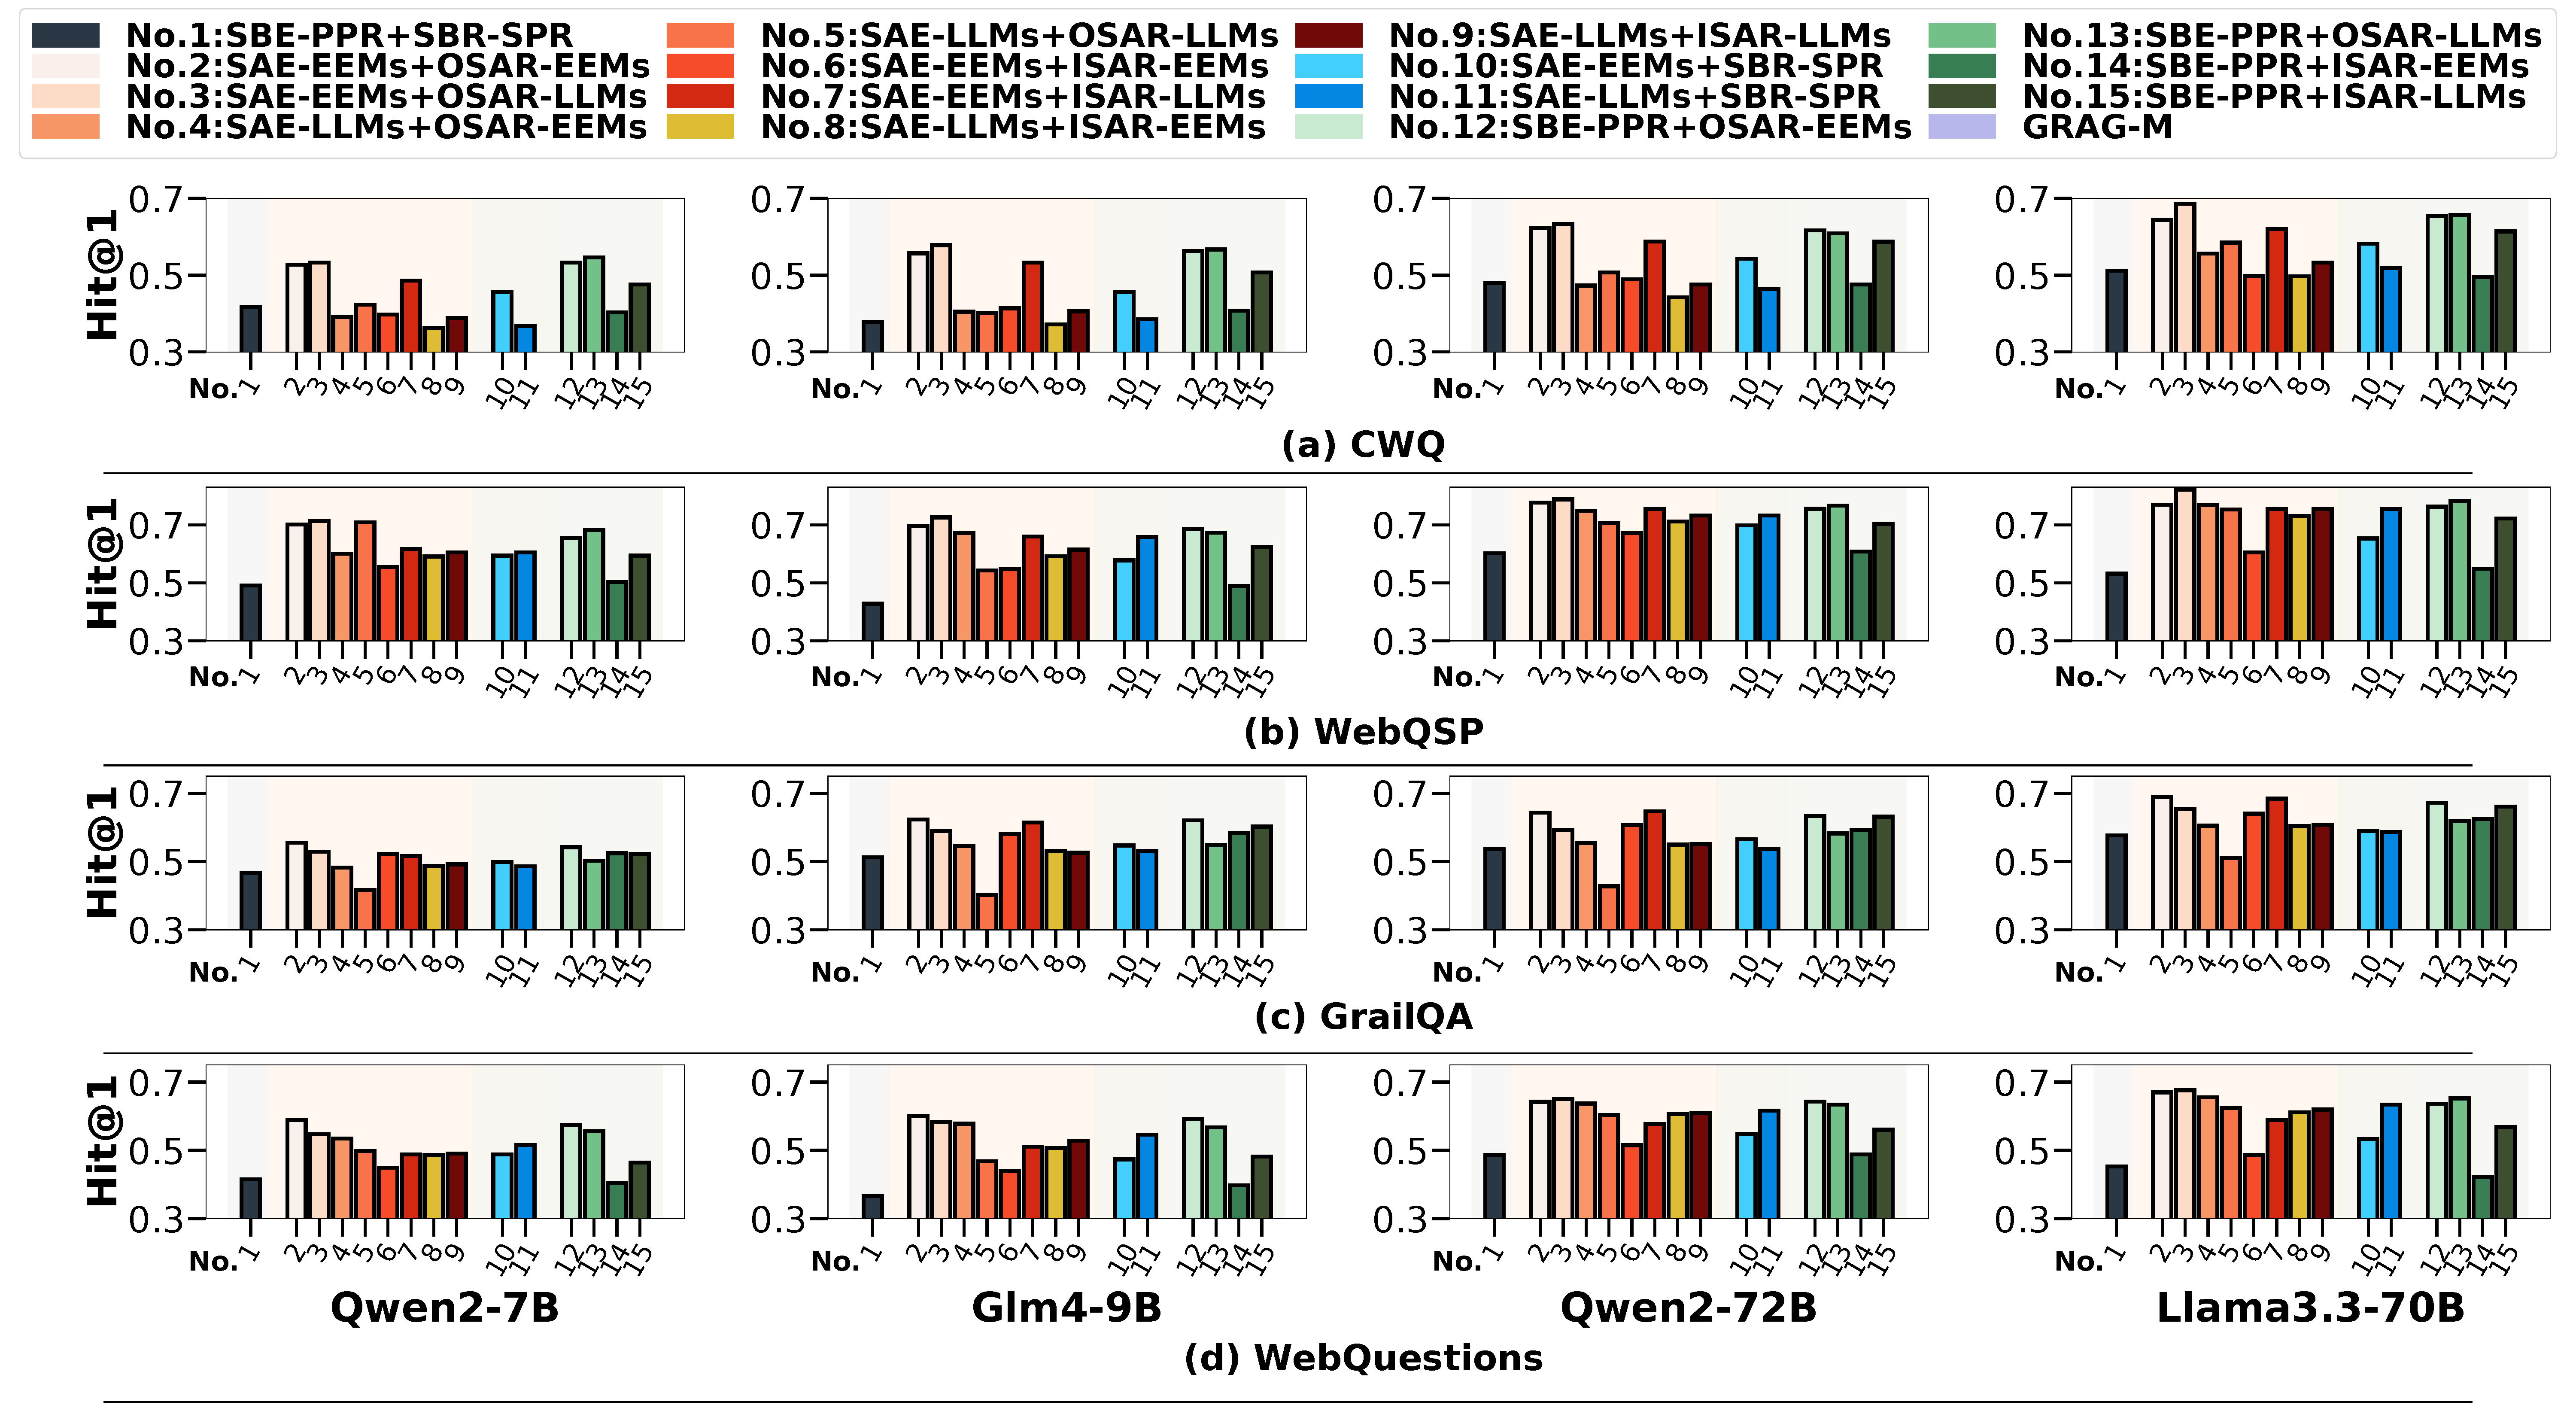
\includegraphics[width=1\textwidth]{figures/Instance/Generation-Hit-32.pdf}
    \vspace{-20pt}
	\caption{\small Reasoning Results of LEGO-GraphRAG Instances Across Four Datasets} 
	\label{fig:Instance}
\end{figure*}

% \begin{comment}
    

% \begin{figure*}[thbp] 
%     \centering
%     \vspace{-10pt}
%     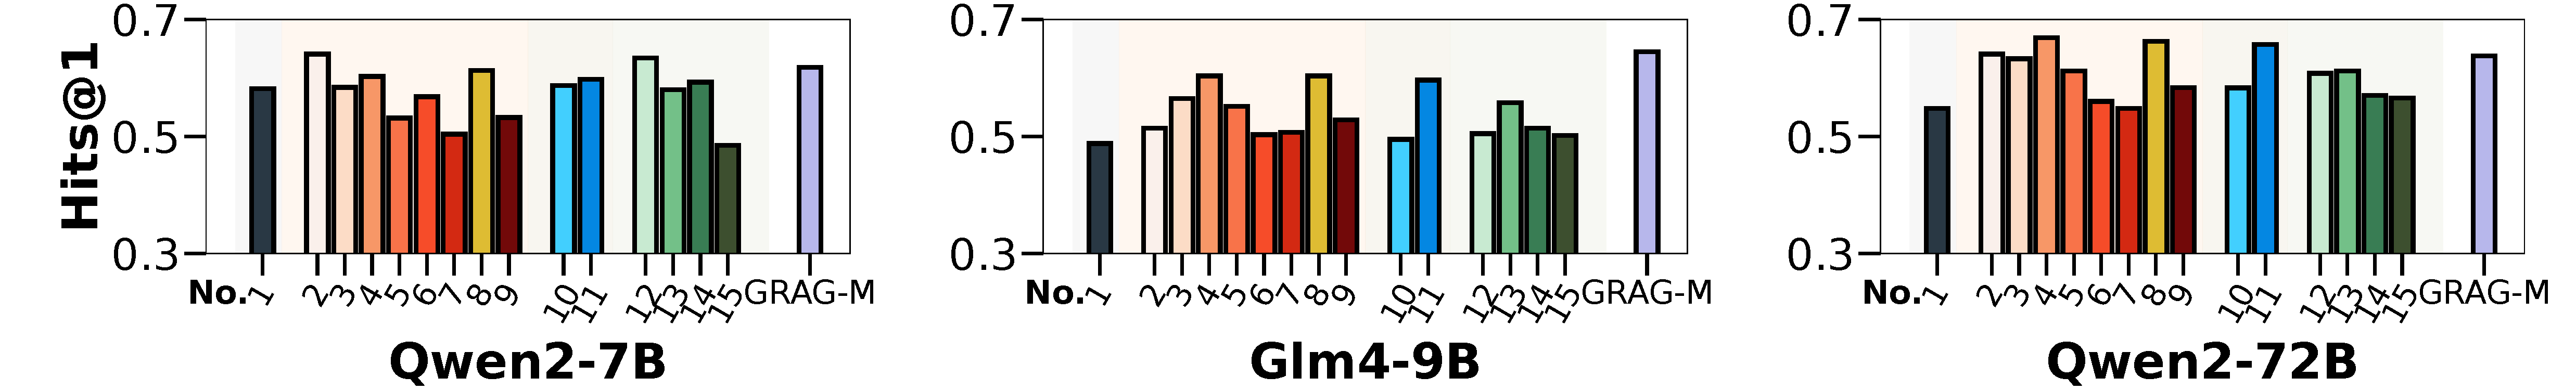
\includegraphics[width=0.73\textwidth]{figures/response/metaQA-16Instance-Generation-Hit32-paper.pdf}
%     \caption{Results of LEGO-GraphRAG and GraphRAG-M Instance on MetaQA Dataset} 
%     \label{fig:GraphRAG-reports}
% \end{figure*}

\begin{figure*}[h!]
    \centering
    \begin{minipage}[b]{0.72\textwidth}
    \centering
    \vspace{-10pt}
    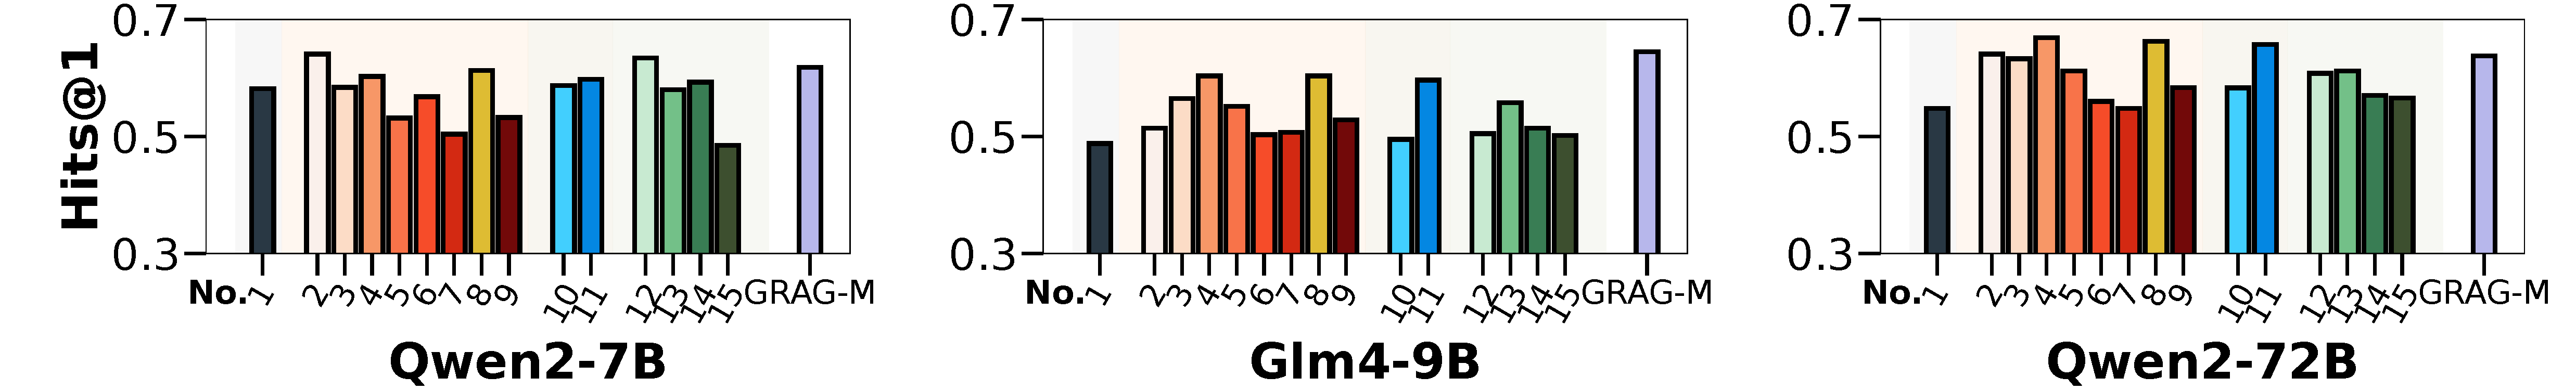
\includegraphics[width=1\textwidth]{figures/response/metaQA-16Instance-Generation-Hit32-paper.pdf}
        \vspace{-20pt}
    \caption{\small Results of LEGO-GraphRAG Instances  and GraphRAG-M Instance on MetaQA Dataset} 
    \label{fig:metaqa}
    \end{minipage}%
    \hspace{0.01\textwidth} 
    \begin{minipage}[b]{0.25\textwidth}
    \centering
    \vspace{-10pt}
    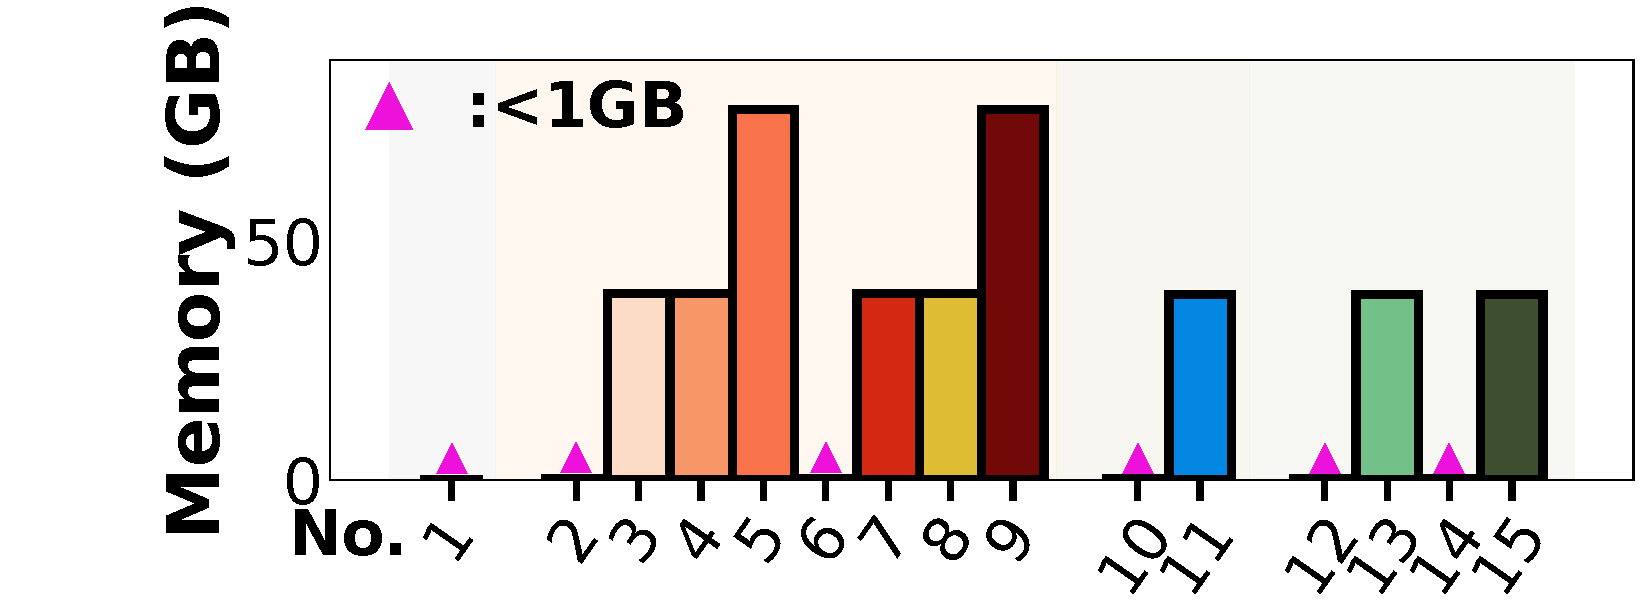
\includegraphics[width=1\textwidth, height = 2.1cm]{figures/Instance/Memory.pdf}
    \vspace{-20pt}
    \caption{\small Peak GPU Memory Usage} 
    \label{fig:GPU}
    \end{minipage}
    \vspace{-10pt}%
\end{figure*}
\vspace{-10pt}
\begin{figure*}[h!]
    \centering
    \begin{minipage}[b]{0.47\textwidth}
        \centering
        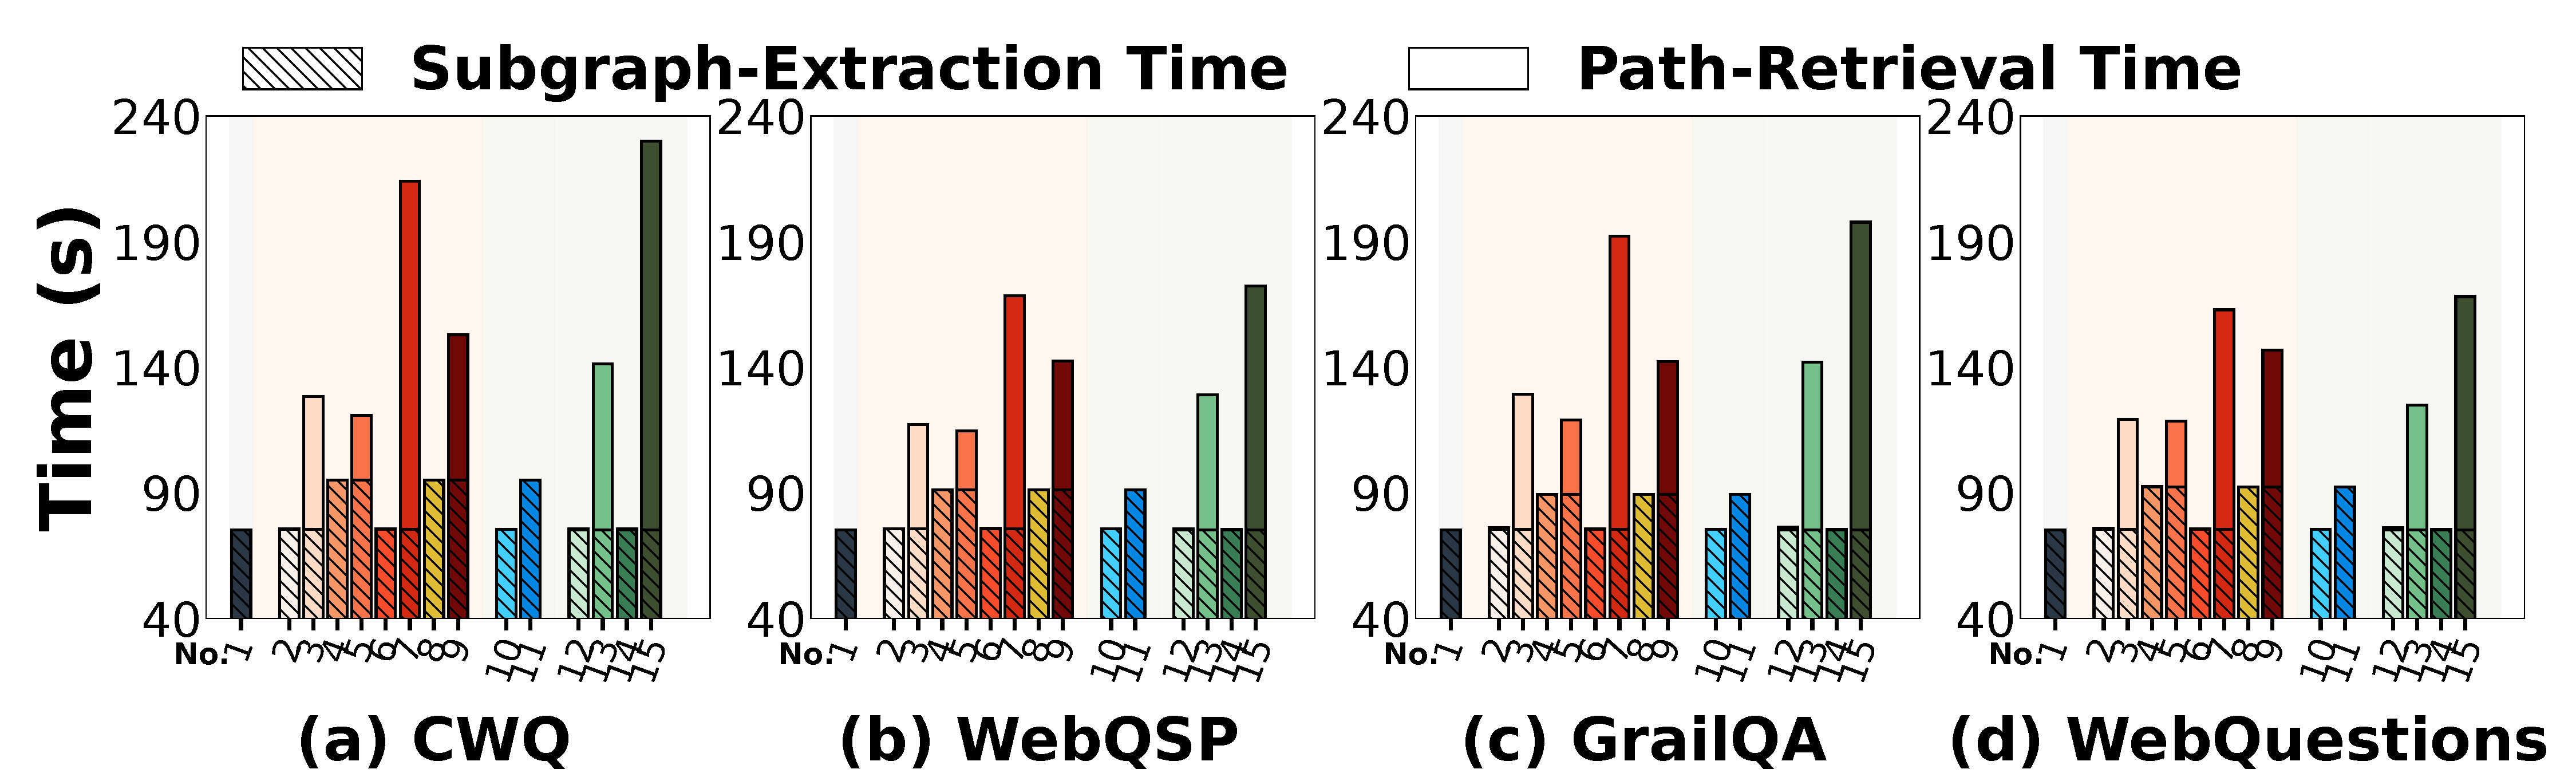
\includegraphics[width=\textwidth]{figures/Instance/Time_INone.pdf}
        \vspace{-20pt}
        \caption{\small Runtime of SE and PR Modules for GraphRAG Instances}
        \label{fig:Instance-time}
    \end{minipage}%
    \hspace{0.01\textwidth} 
    \begin{minipage}[b]{0.47\textwidth}
        \centering
        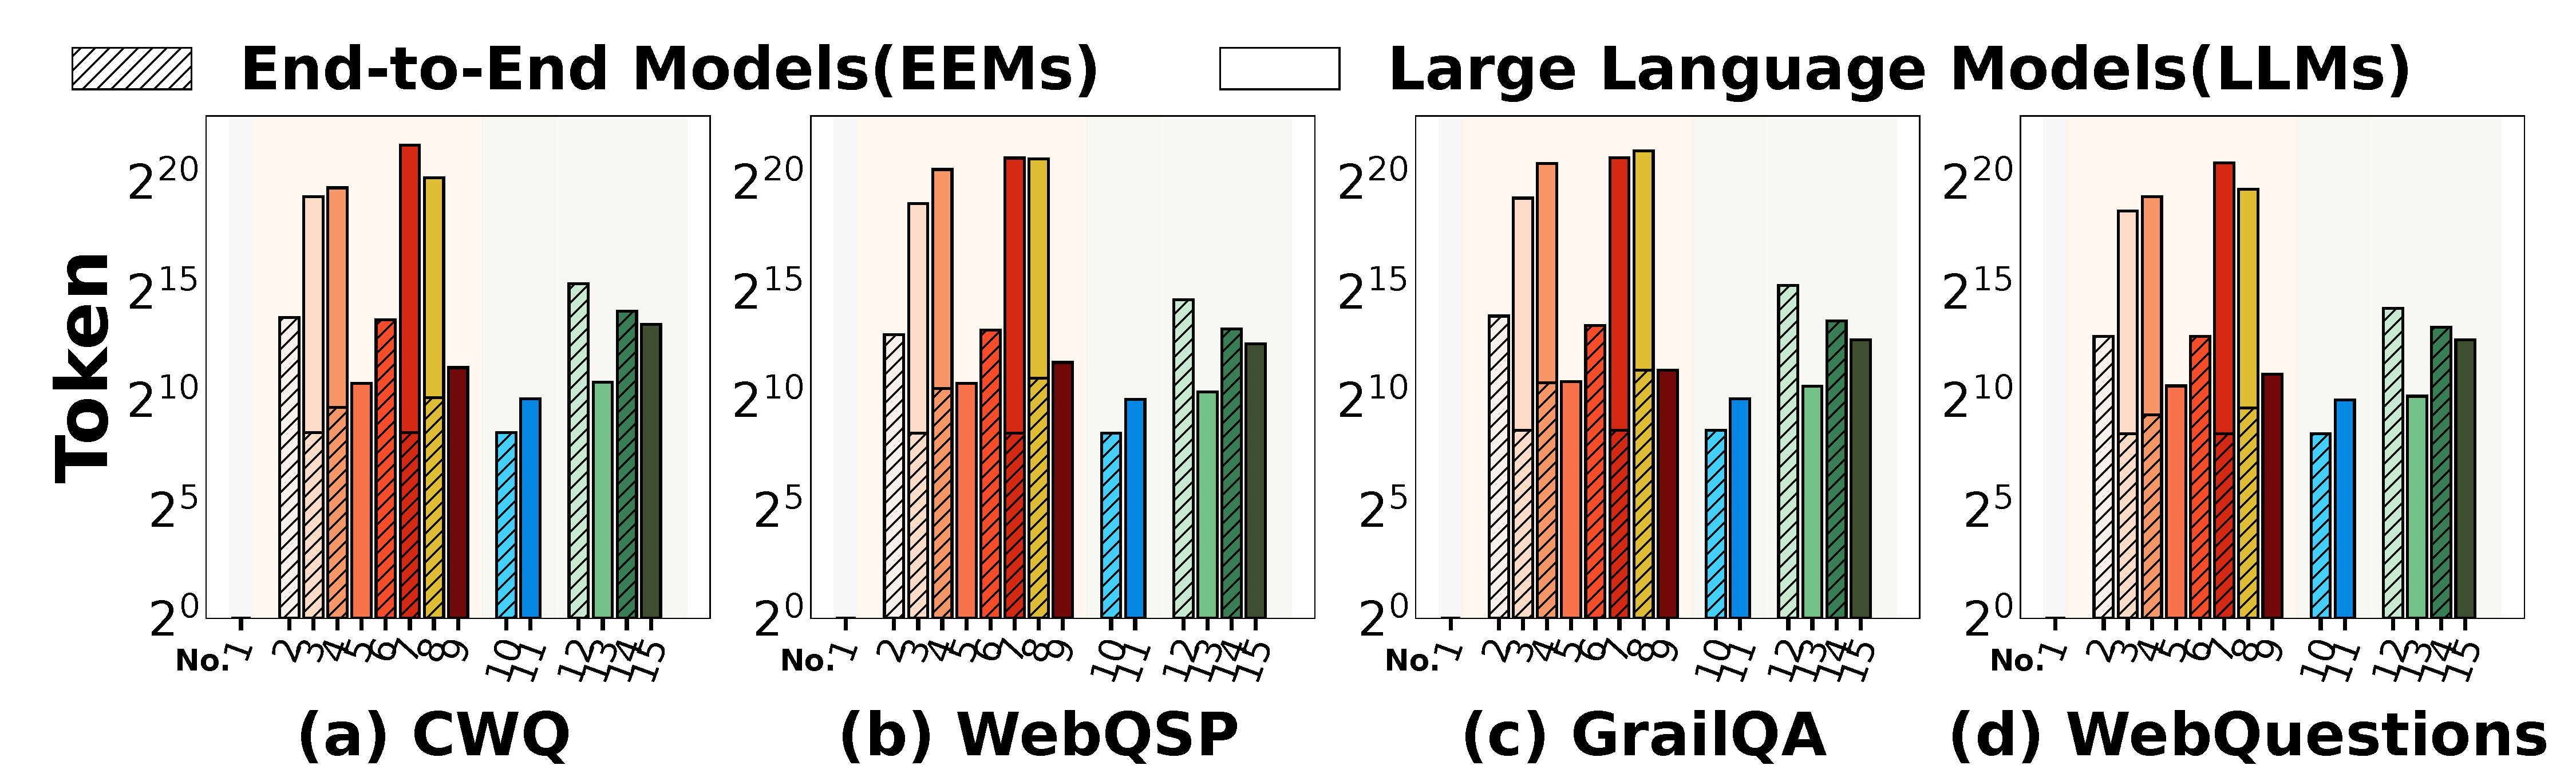
\includegraphics[width=\textwidth]{figures/Instance/Token_INone.pdf}
         \vspace{-20pt}
        \caption{\small Token Costs for EEMs and LLMs in GraphRAG Instances}
        \label{fig:Instance-token}
    \end{minipage}%
    \vspace{-10pt}
\end{figure*}


% \begin{figure*}[h!]
%     \centering
%     \begin{minipage}[b]{0.47\textwidth}
%         \centering
%         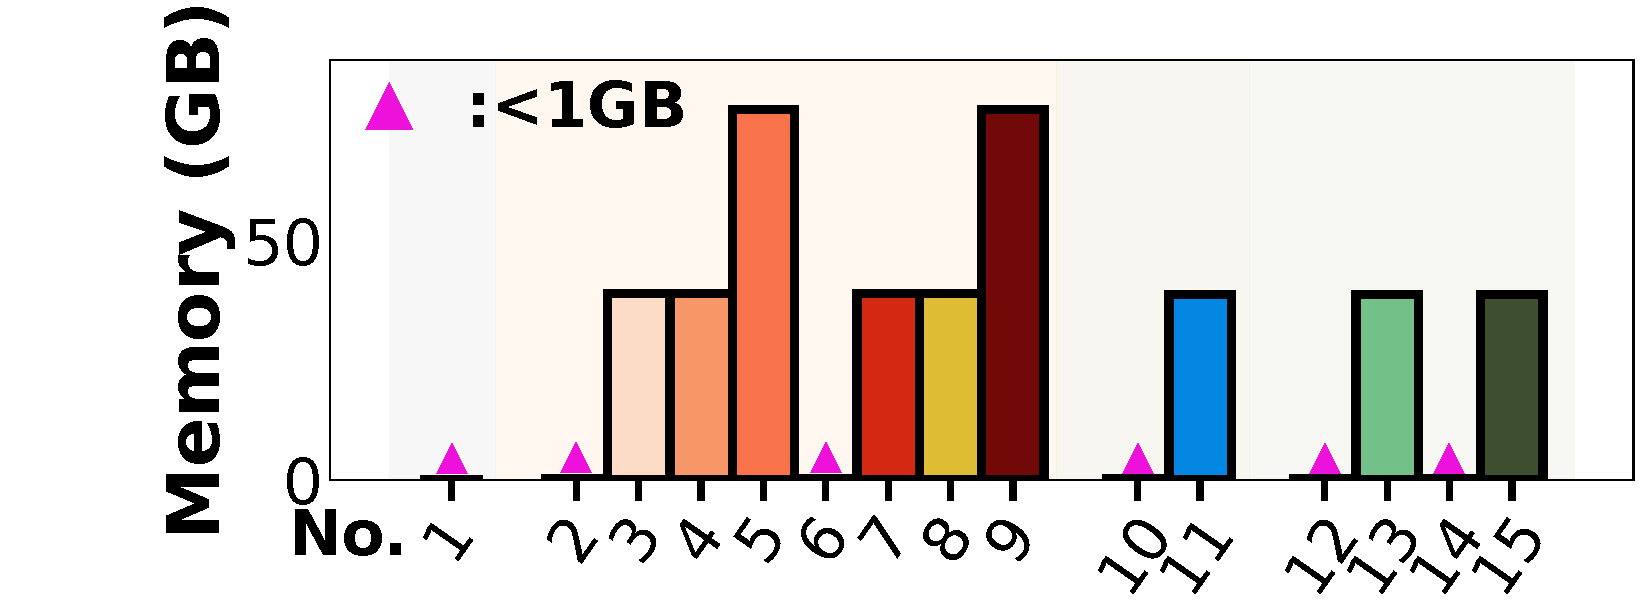
\includegraphics[width=\textwidth]{figures/Instance/Memory.pdf}
%         % \vspace{-10pt}
%         \caption{Peak GPU Memory Usage of GraphRAG Instances}
%         % \vspace{-10pt}
%         \label{fig:GPU}
%     \end{minipage}%
%     \hspace{0.01\textwidth} 
%     \begin{minipage}[b]{0.47\textwidth} 
%         \centering  
%         \begin{subfigure}{1\textwidth}  
%             \centering  
%             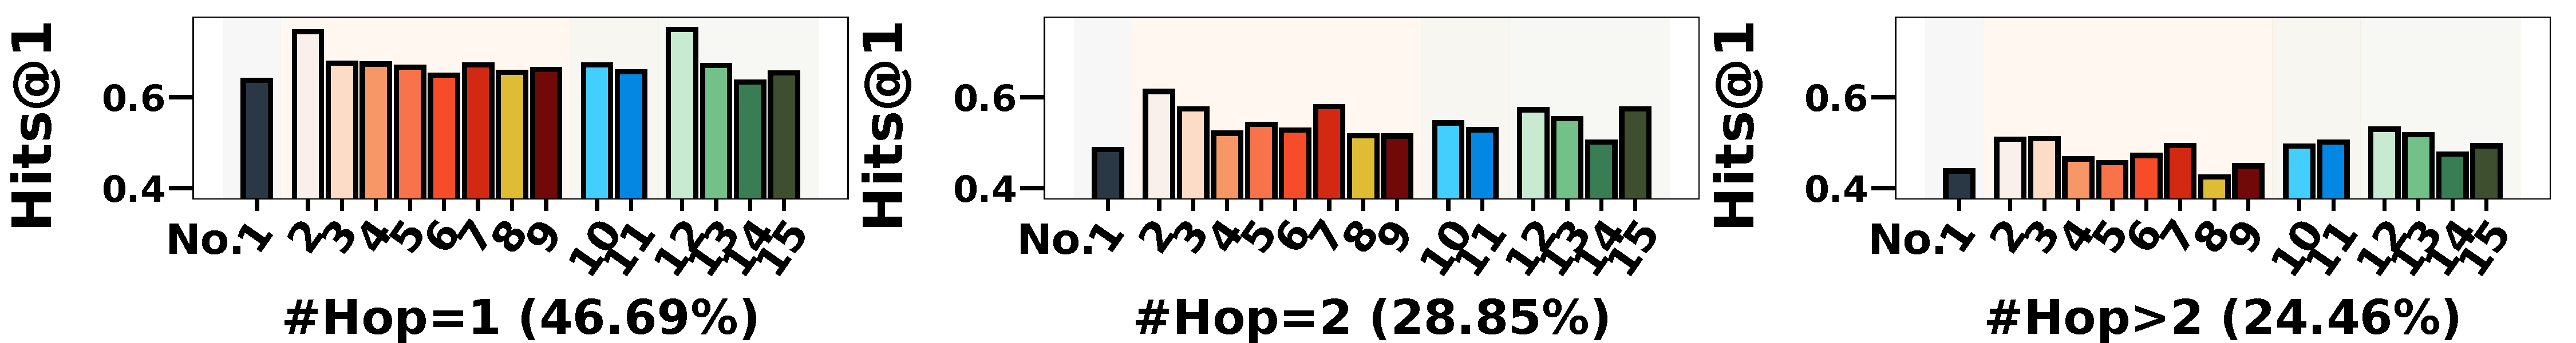
\includegraphics[width=\textwidth]{figures/response/Average-Hop-Hit32.pdf}  
%             \\[-0.5em]
%             \caption{Classifying queries by the number of reasoning hops}  
%             \label{fig:Hop}  
%         \end{subfigure}  
        
%         % \hfill  
%         \begin{subfigure}{1\textwidth}  
%             \centering  
%             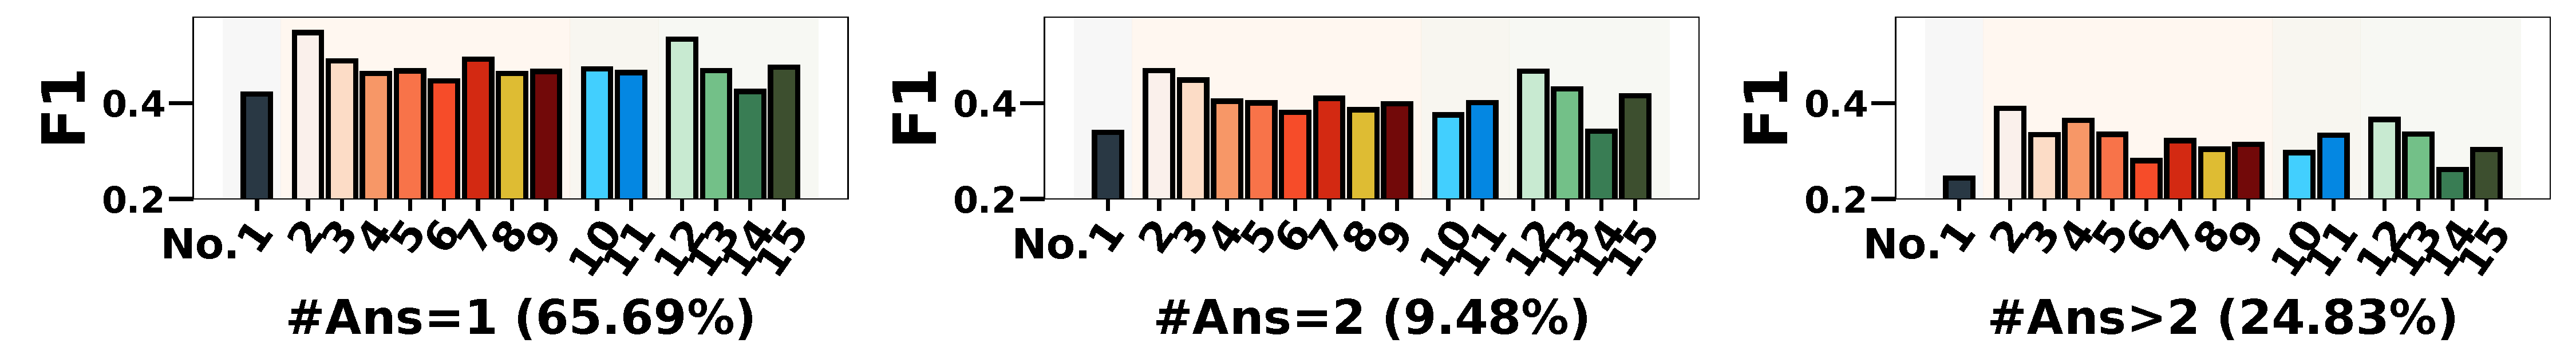
\includegraphics[width=\textwidth]{figures/response/Average-Answer-F132.pdf}  
%             \\[-0.5em]
%             \caption{Classifying queries by the number of answers}  
%             \label{fig:Answer}  
%         \end{subfigure}  
        
%         \begin{subfigure}{1\textwidth}  
%             \centering  
%             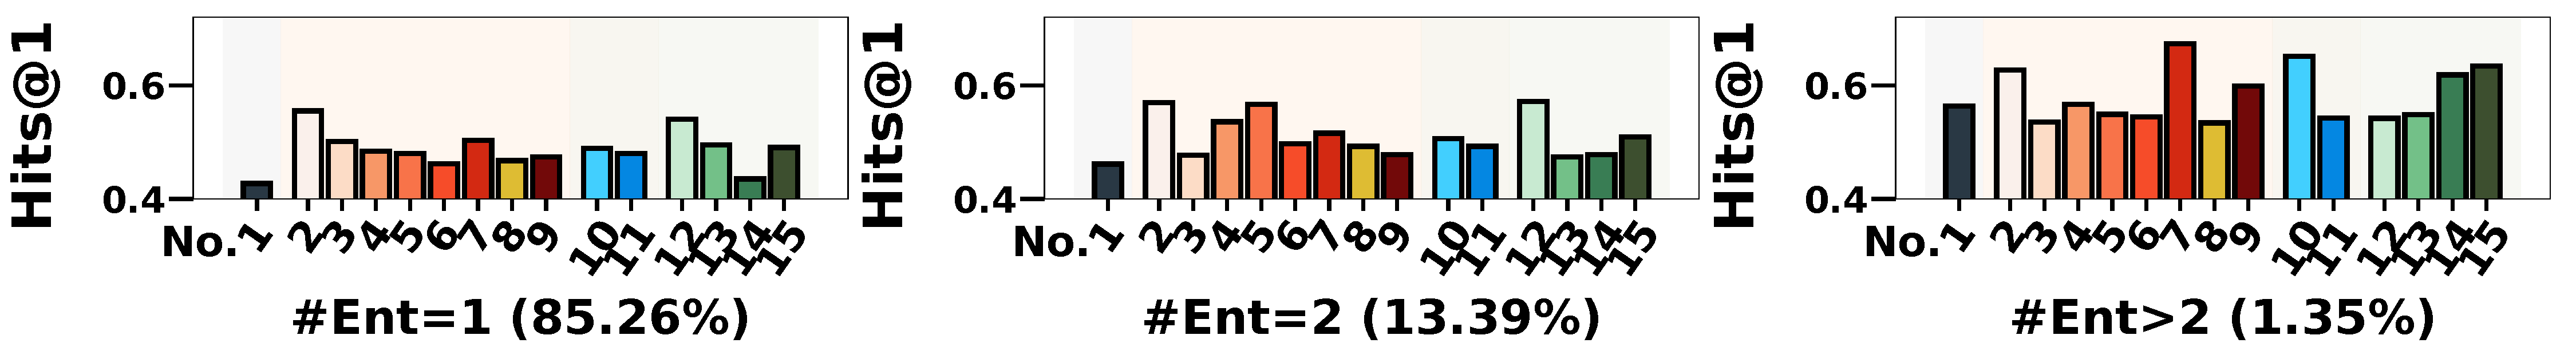
\includegraphics[width=\textwidth]{figures/response/Average-Entity-Hit32.pdf}  
%             \caption{Classifying queries by the number of entities}  
%             \label{fig:Entity}  
%         \end{subfigure}  
%         \\[-1em]
%         \caption{Performance of LEGO-GraphRAG Instances Under Different Classification of Queries}
%         \label{fig:combined}  
%     \end{minipage}%
% \end{figure*}
% \begin{figure}[t] 
%     \centering
%     \vspace{-10pt}
%     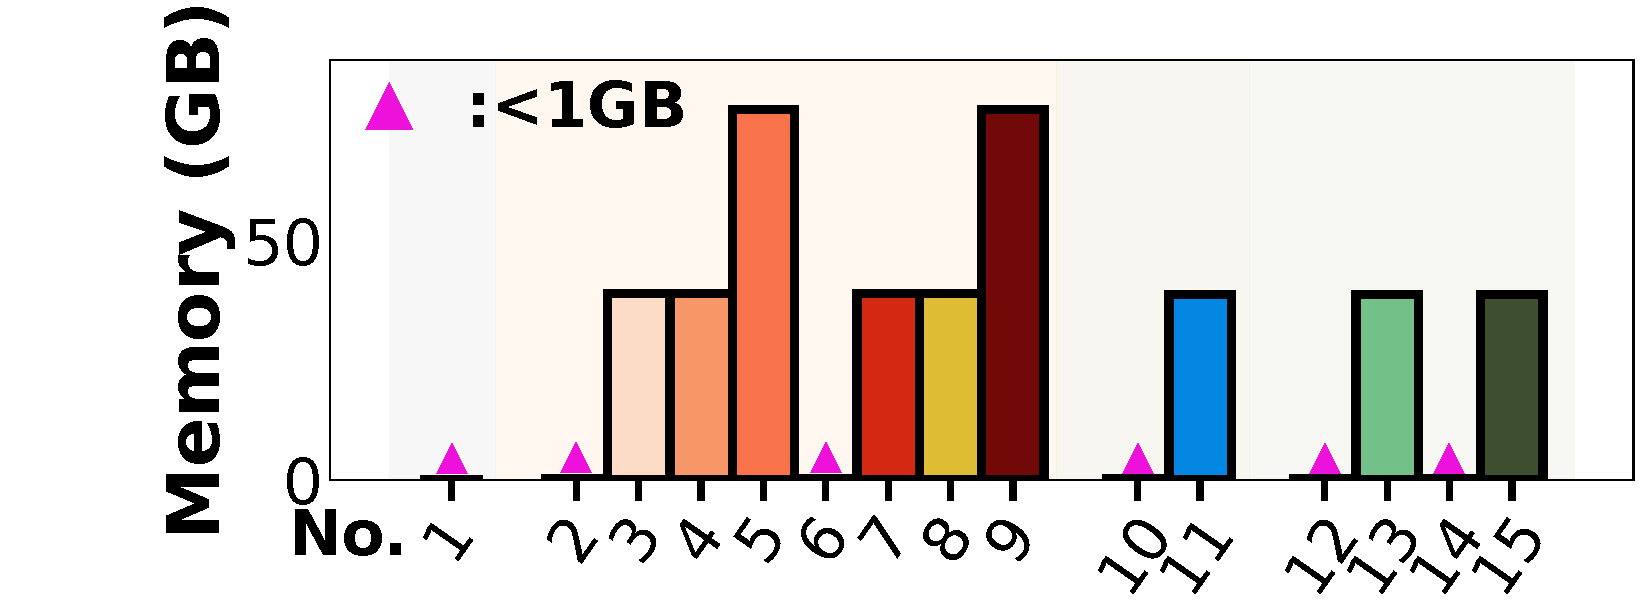
\includegraphics[width=0.24\textwidth]{figures/Instance/Memory.pdf}
%     \vspace{-10pt}
%     \caption{Peak GPU Memory Usage of GraphRAG Instances} 
%     \label{fig:GPU}
%         \vspace{-5pt}
% \end{figure}

\begin{figure}[h!]  
    \centering  
    \begin{subfigure}{0.48\textwidth}  
        \centering  
        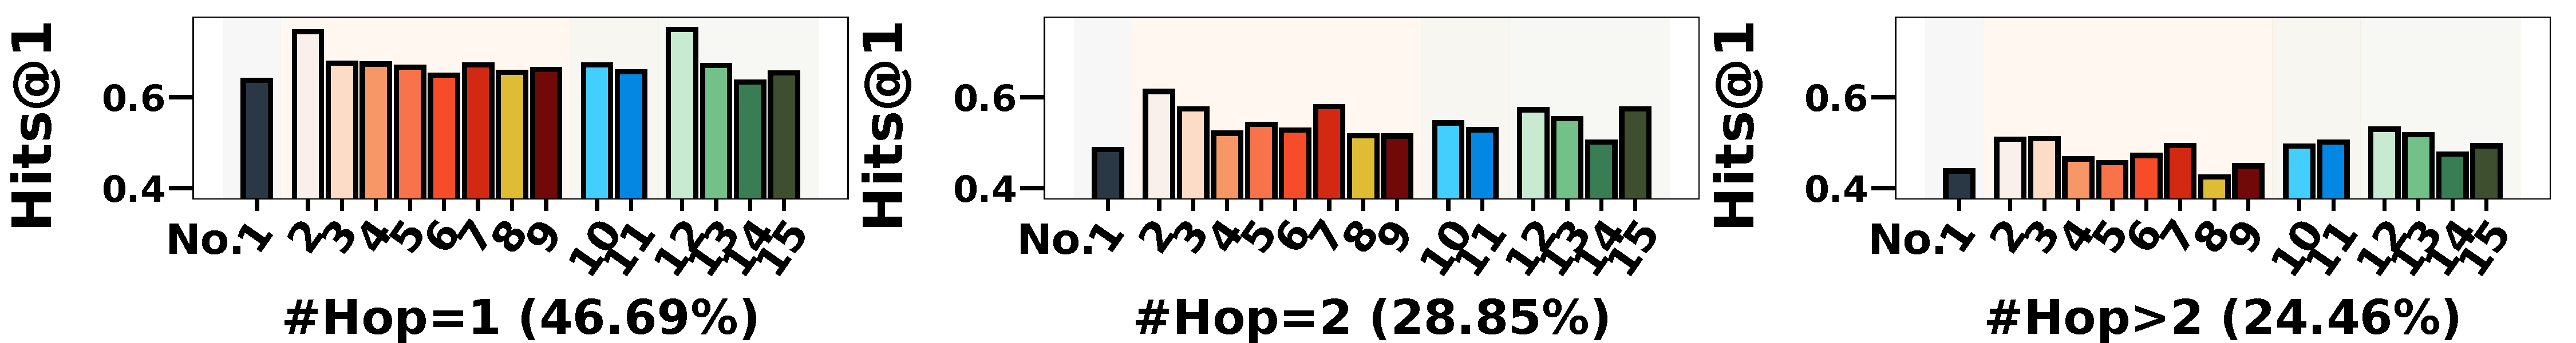
\includegraphics[width=\textwidth]{figures/response/Average-Hop-Hit32.pdf}  
         %       \vspace{-5pt}
        %\caption{\small Classifying queries by the number of reasoning hops}  
        \caption{\small Queries with Varied Number of Reasoning Hops} 
        \label{fig:Hop}  
    \end{subfigure}  
    %\vspace{-5pt}
    \begin{subfigure}{0.48\textwidth}  
        \centering  
        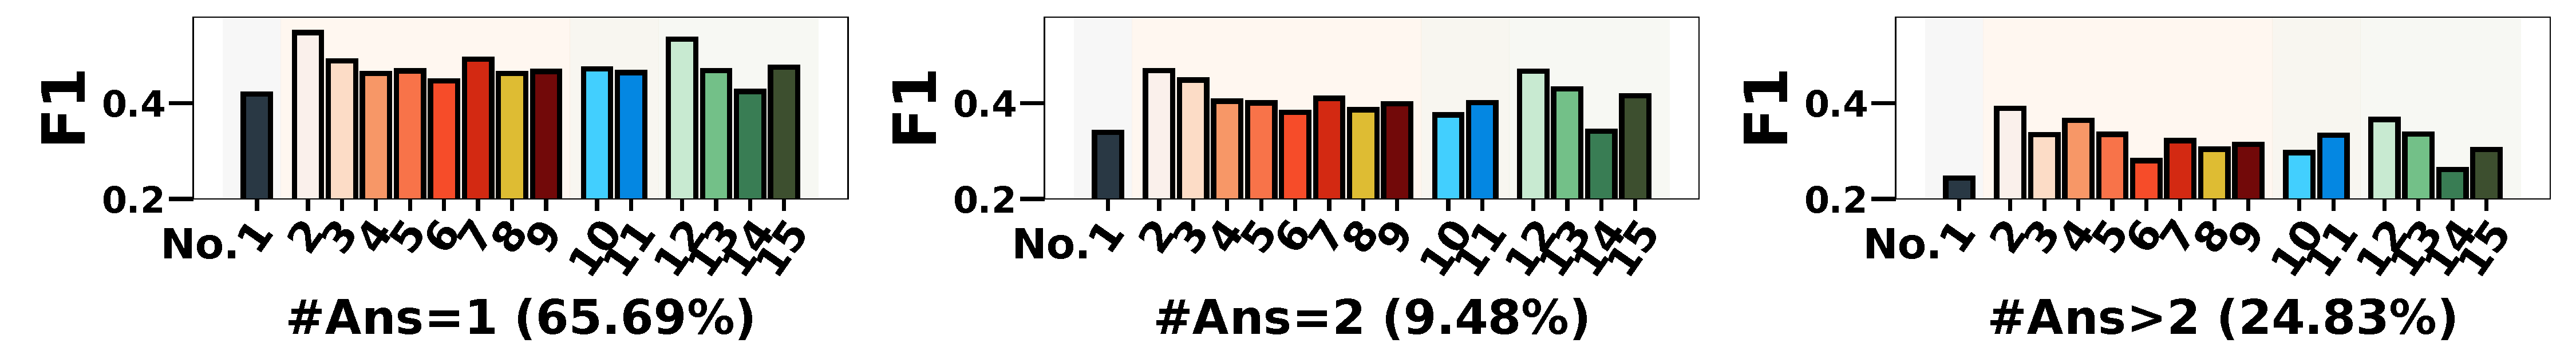
\includegraphics[width=\textwidth]{figures/response/Average-Answer-F132.pdf}  
          %      \vspace{-5pt}
        %\caption{\small Classifying queries by the number of answers}  
                \caption{\small Queries with Varied Number of Answers}
        \label{fig:Answer}  
    \end{subfigure}  
    %\vspace{-5pt}
    \begin{subfigure}{0.48\textwidth}  
        \centering  
        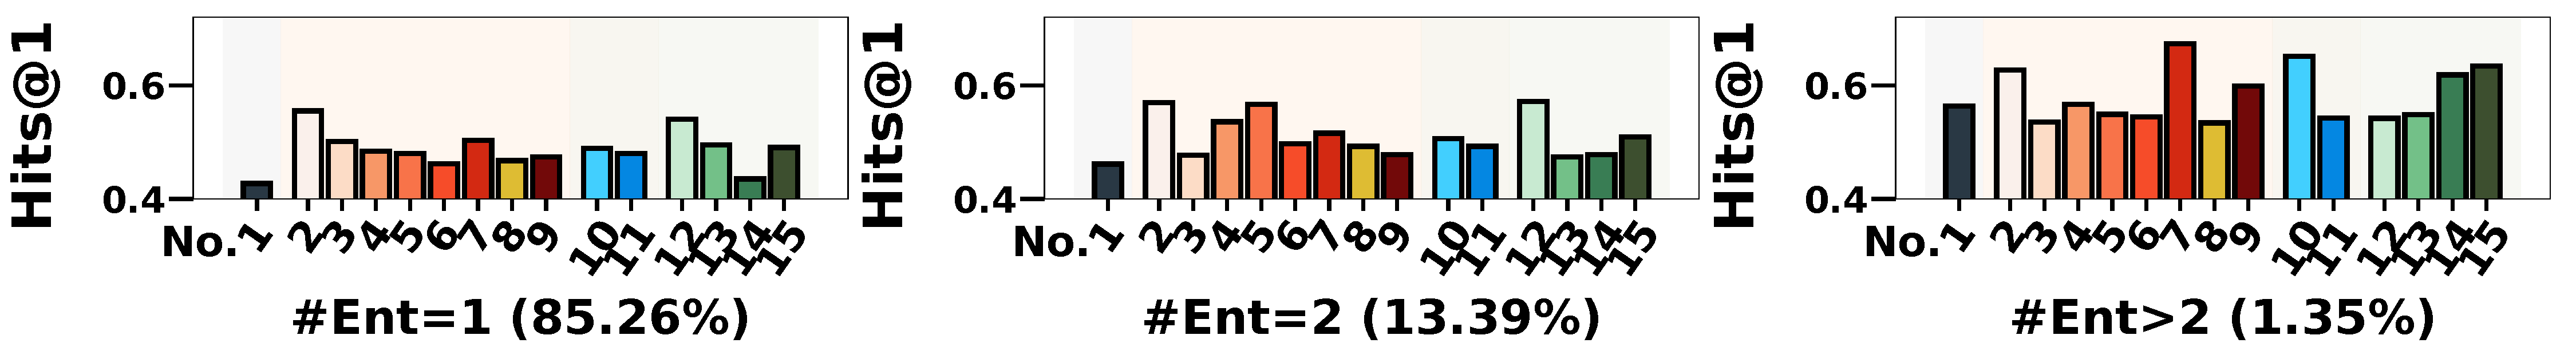
\includegraphics[width=\textwidth]{figures/response/Average-Entity-Hit32.pdf}
        %\vspace{-5pt}
        %\caption{\small Classifying queries by the number of entities}  
                \caption{\small Queries with Varied Number of Entities}
        \label{fig:Entity}  
    \end{subfigure}  
    \vspace{-22pt}
    %\caption{Performance of LEGO-GraphRAG Instances Under Different Classification of Queries}
    \caption{Instance Performance w.r.t. Queries}
    \label{fig:combined}  
   \vspace{-8pt}
\end{figure} 
% \begin{minipage}[b]{0.73\textwidth} 
%     \centering  
%     \begin{subfigure}{0.48\textwidth}  
%         \centering  
%         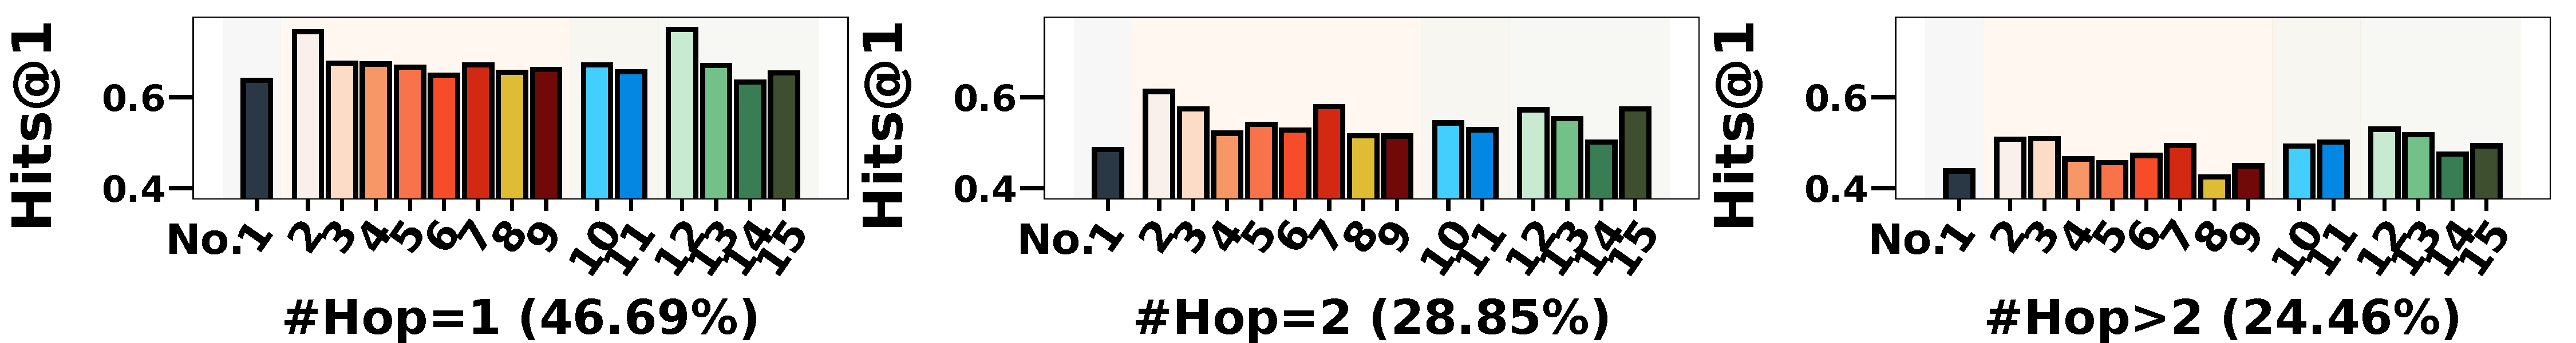
\includegraphics[width=\textwidth]{figures/response/Average-Hop-Hit32.pdf}  
%         \caption{Classifying queries by the number of reasoning hops}  
%         \label{fig:Hop}  
%     \end{subfigure}  
%     \hfill  
%     \begin{subfigure}{0.48\textwidth}  
%         \centering  
%         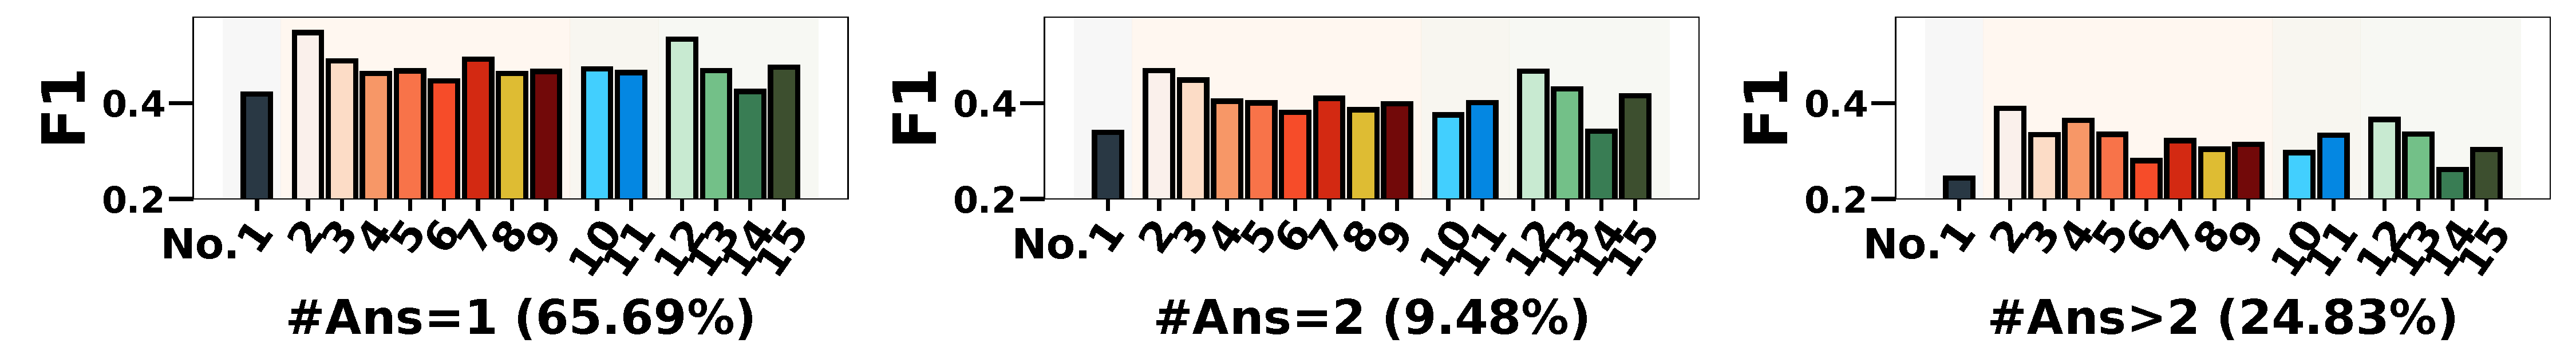
\includegraphics[width=\textwidth]{figures/response/Average-Answer-F132.pdf}  
%         \caption{Classifying queries by the number of answers}  
%         \label{fig:Answer}  
%     \end{subfigure}  
    
%     \begin{subfigure}{0.48\textwidth}  
%         \centering  
%         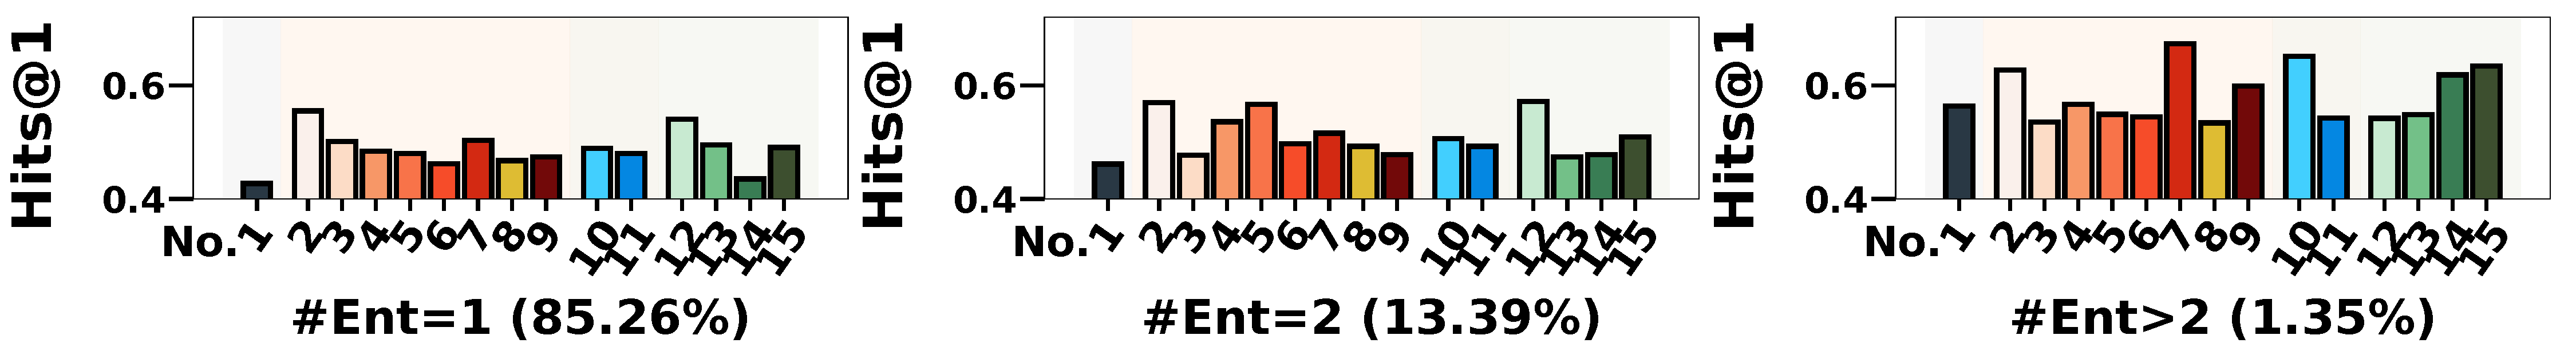
\includegraphics[width=\textwidth]{figures/response/Average-Entity-Hit32.pdf}  
%         \caption{Classifying queries by the number of entities}  
%         \label{fig:Entity}  
%     \end{subfigure}  
    
%     \caption{Performance of LEGO-GraphRAG Instances Under Different Classification of Queries}
%     \label{fig:combined}  
% \end{minipage}%

\begin{comment}

\end{comment}

\begin{comment}
    
\begin{figure}[t] 
    \centering
    \vspace{-10pt}
    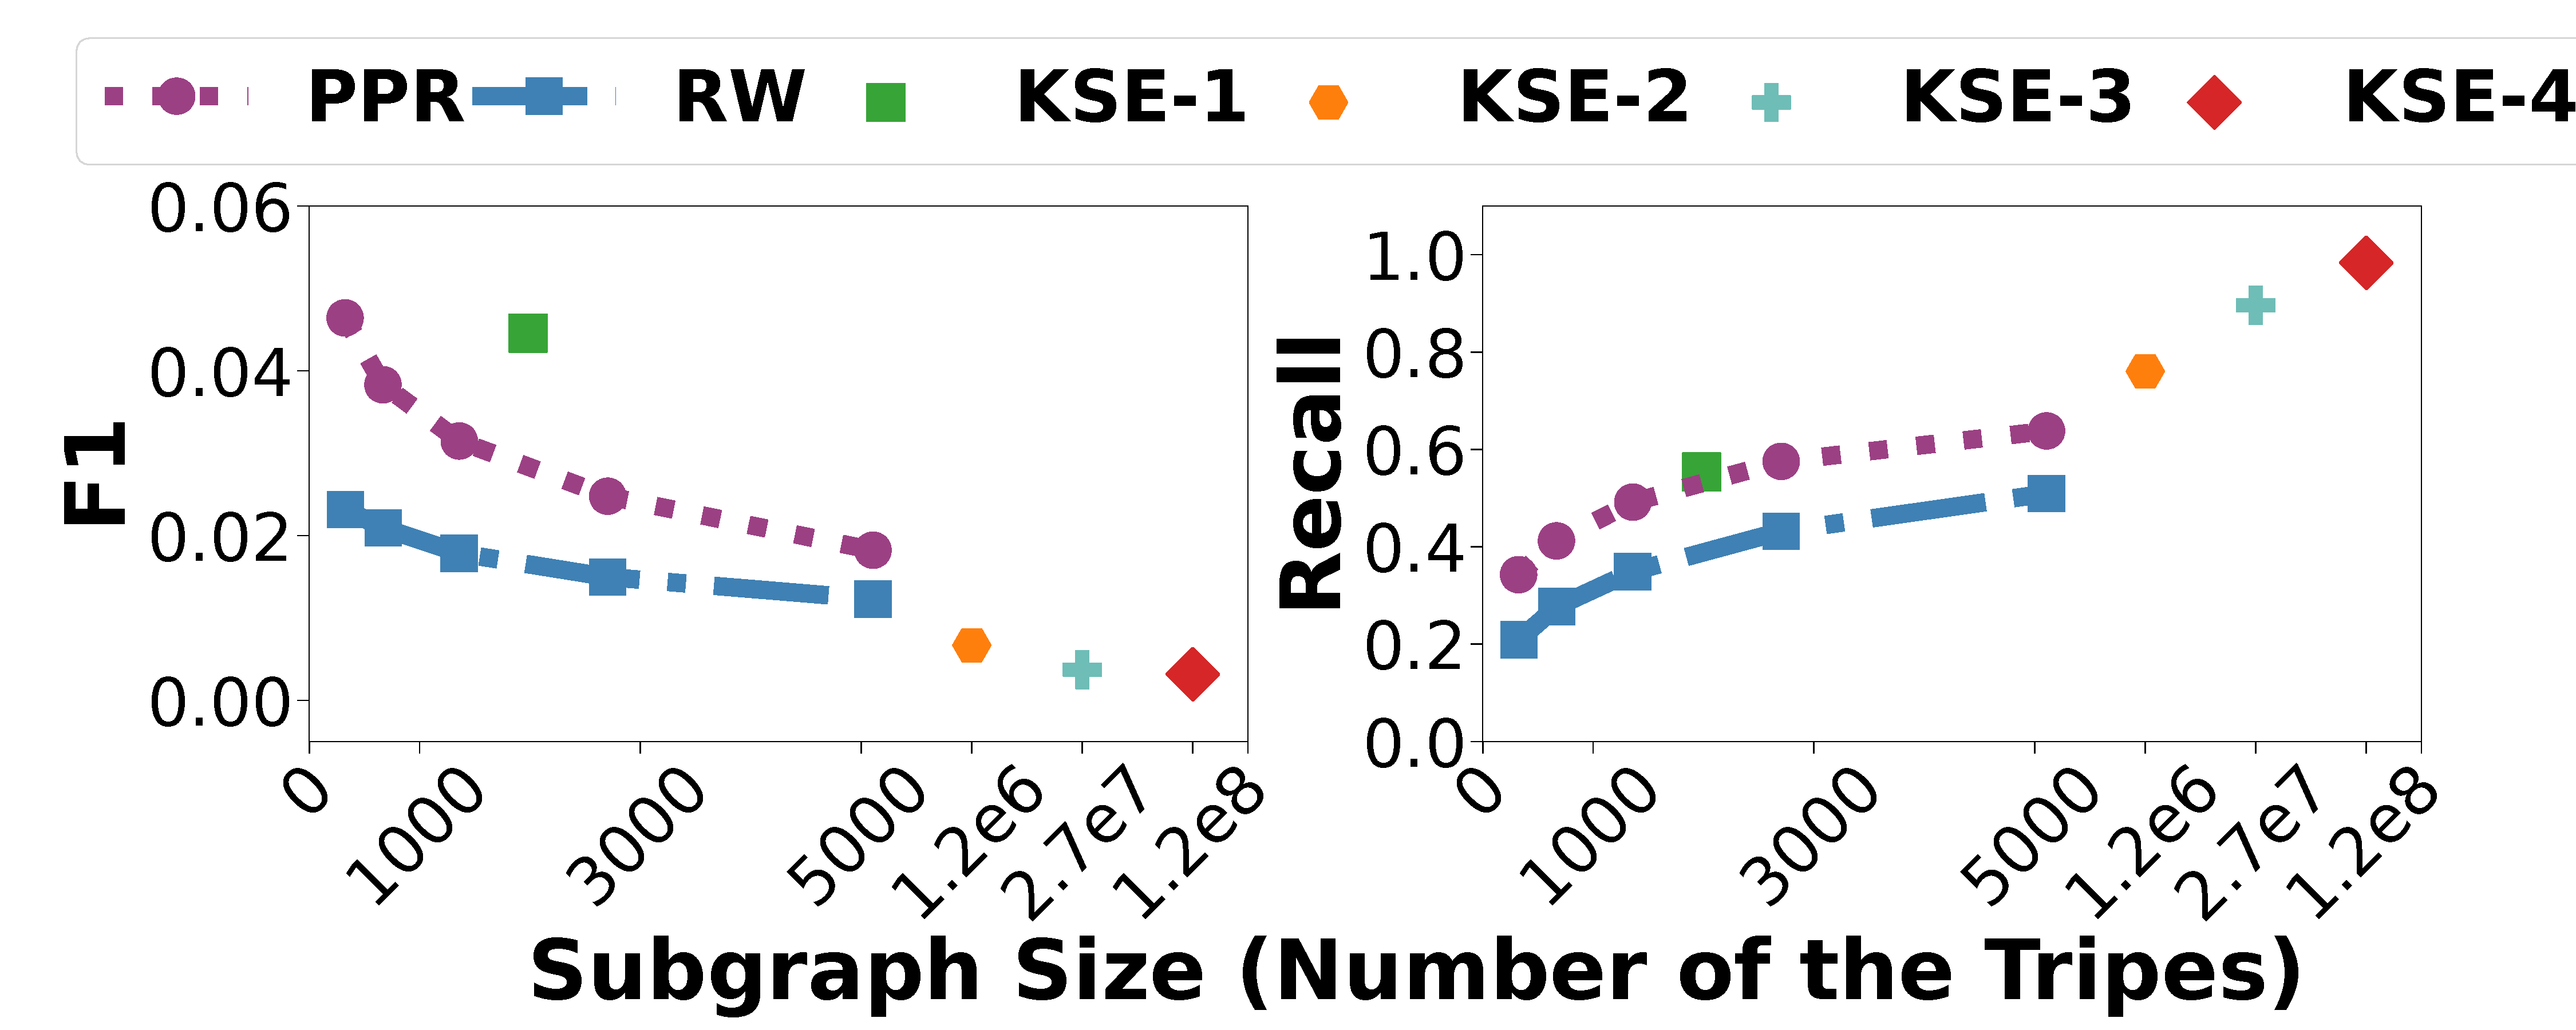
\includegraphics[width=0.48\textwidth]{figures/SE/StructModel.pdf}
    \vspace{-20pt}
    \caption{Recall, F1 Score w.r.t. Subgraph Size in SBE Methods} 
    \label{fig:SE-structmodel}
        \vspace{-5pt}
\end{figure}

\begin{figure}[t] 
    \centering
    \vspace{-10pt}
    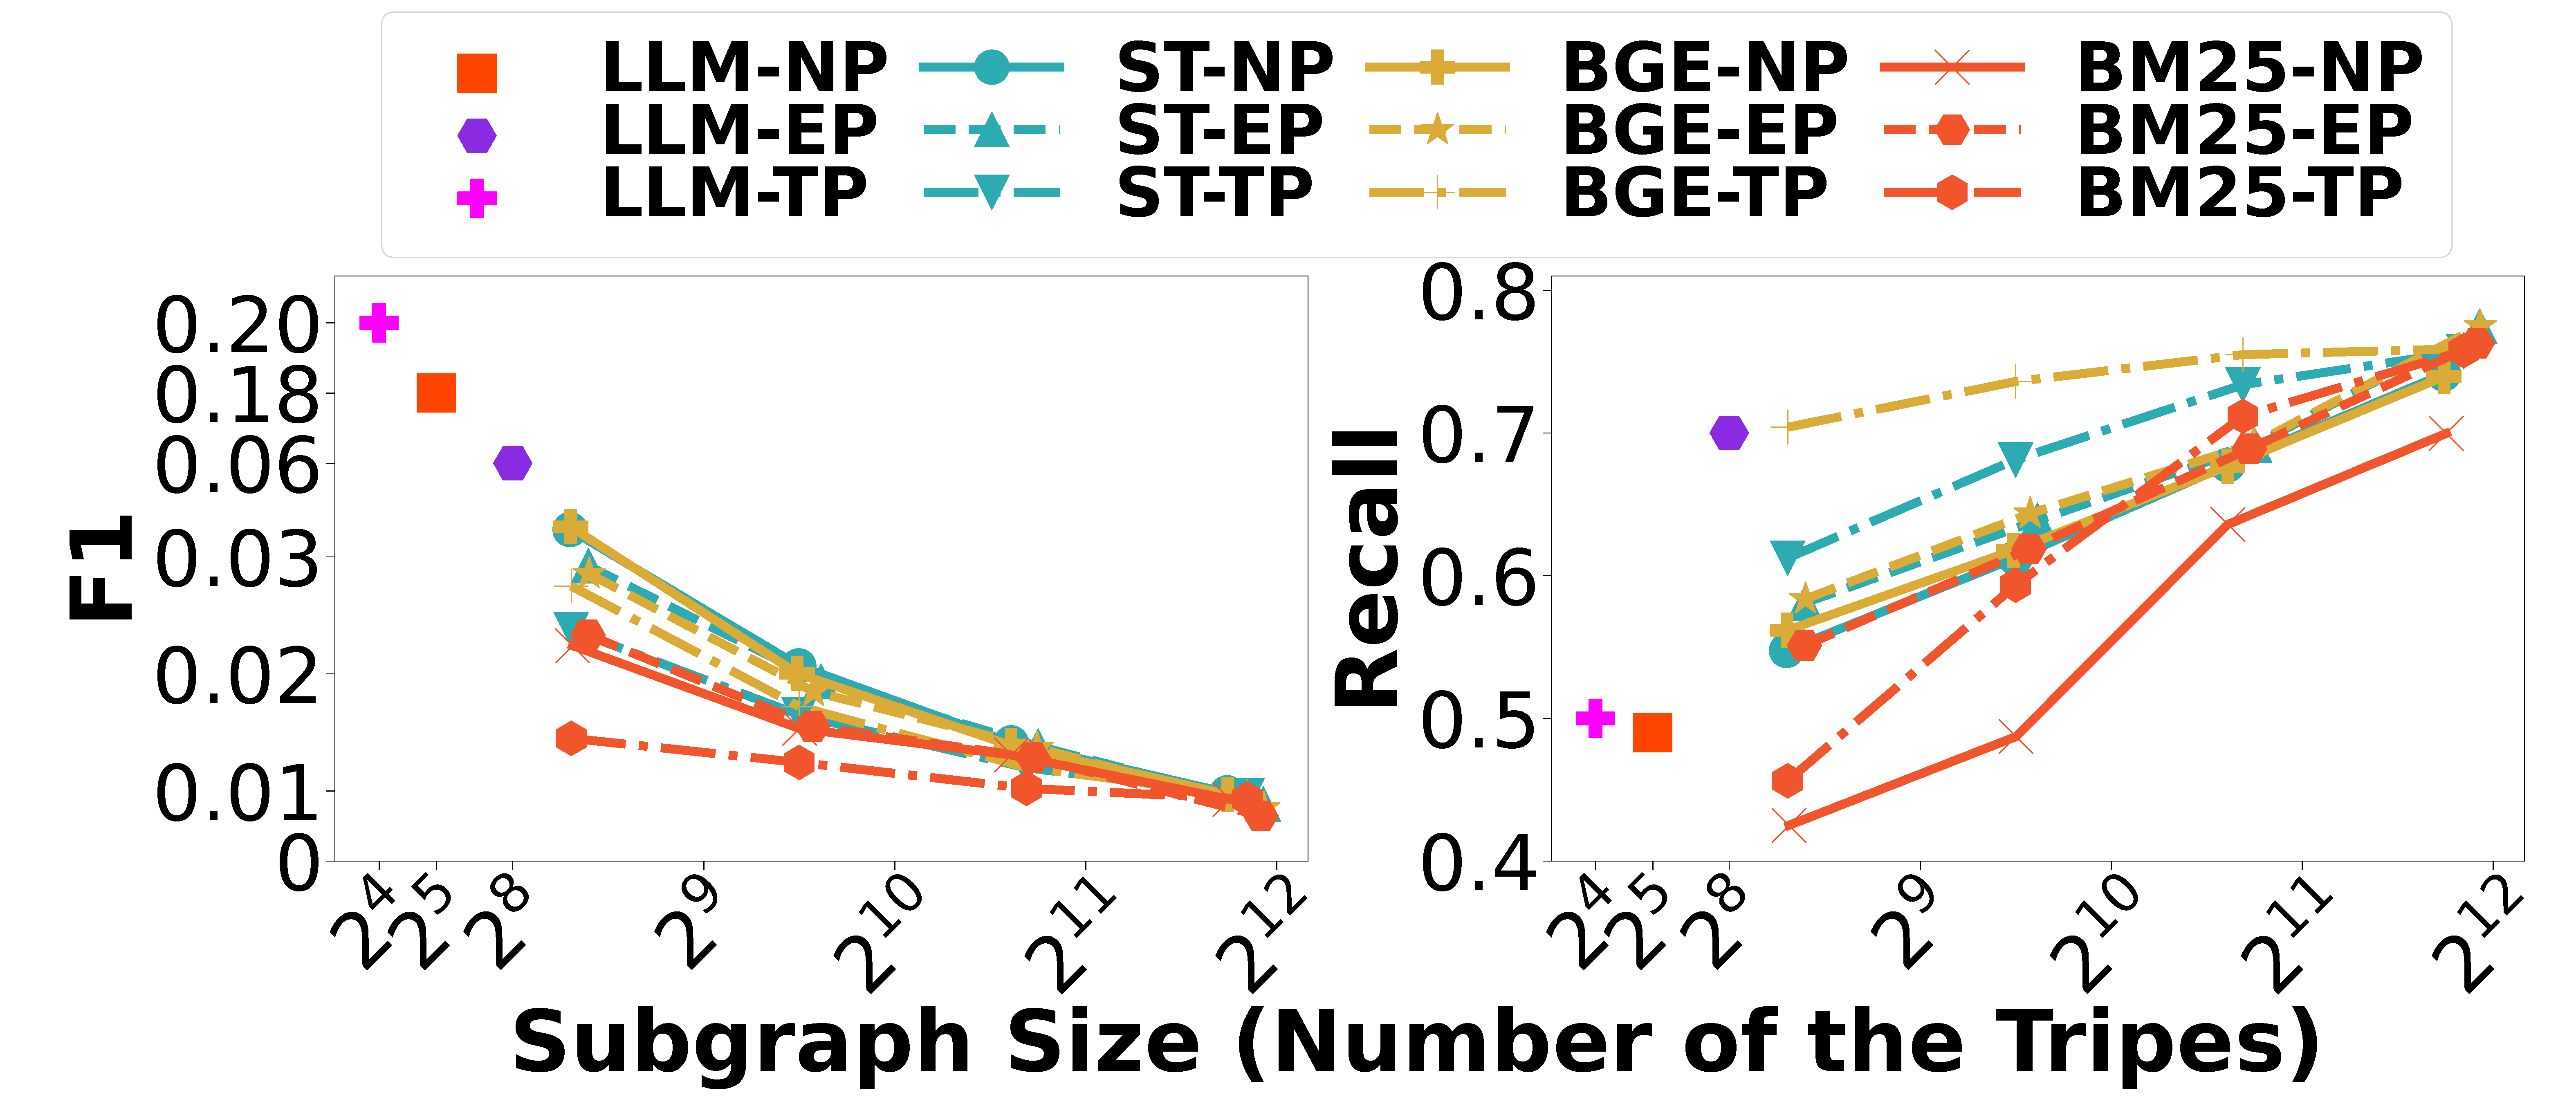
\includegraphics[width=0.48\textwidth]{figures/SE/SmallModel.pdf}
    \vspace{-22pt}
    \caption{Recall, F1 Score w.r.t. Subgraph Size in SAE Methods} 
    \label{fig:se-smallmodel}
    \vspace{-3pt}
\end{figure}

\begin{figure}[t] 
    \centering
    \vspace{-10pt}
    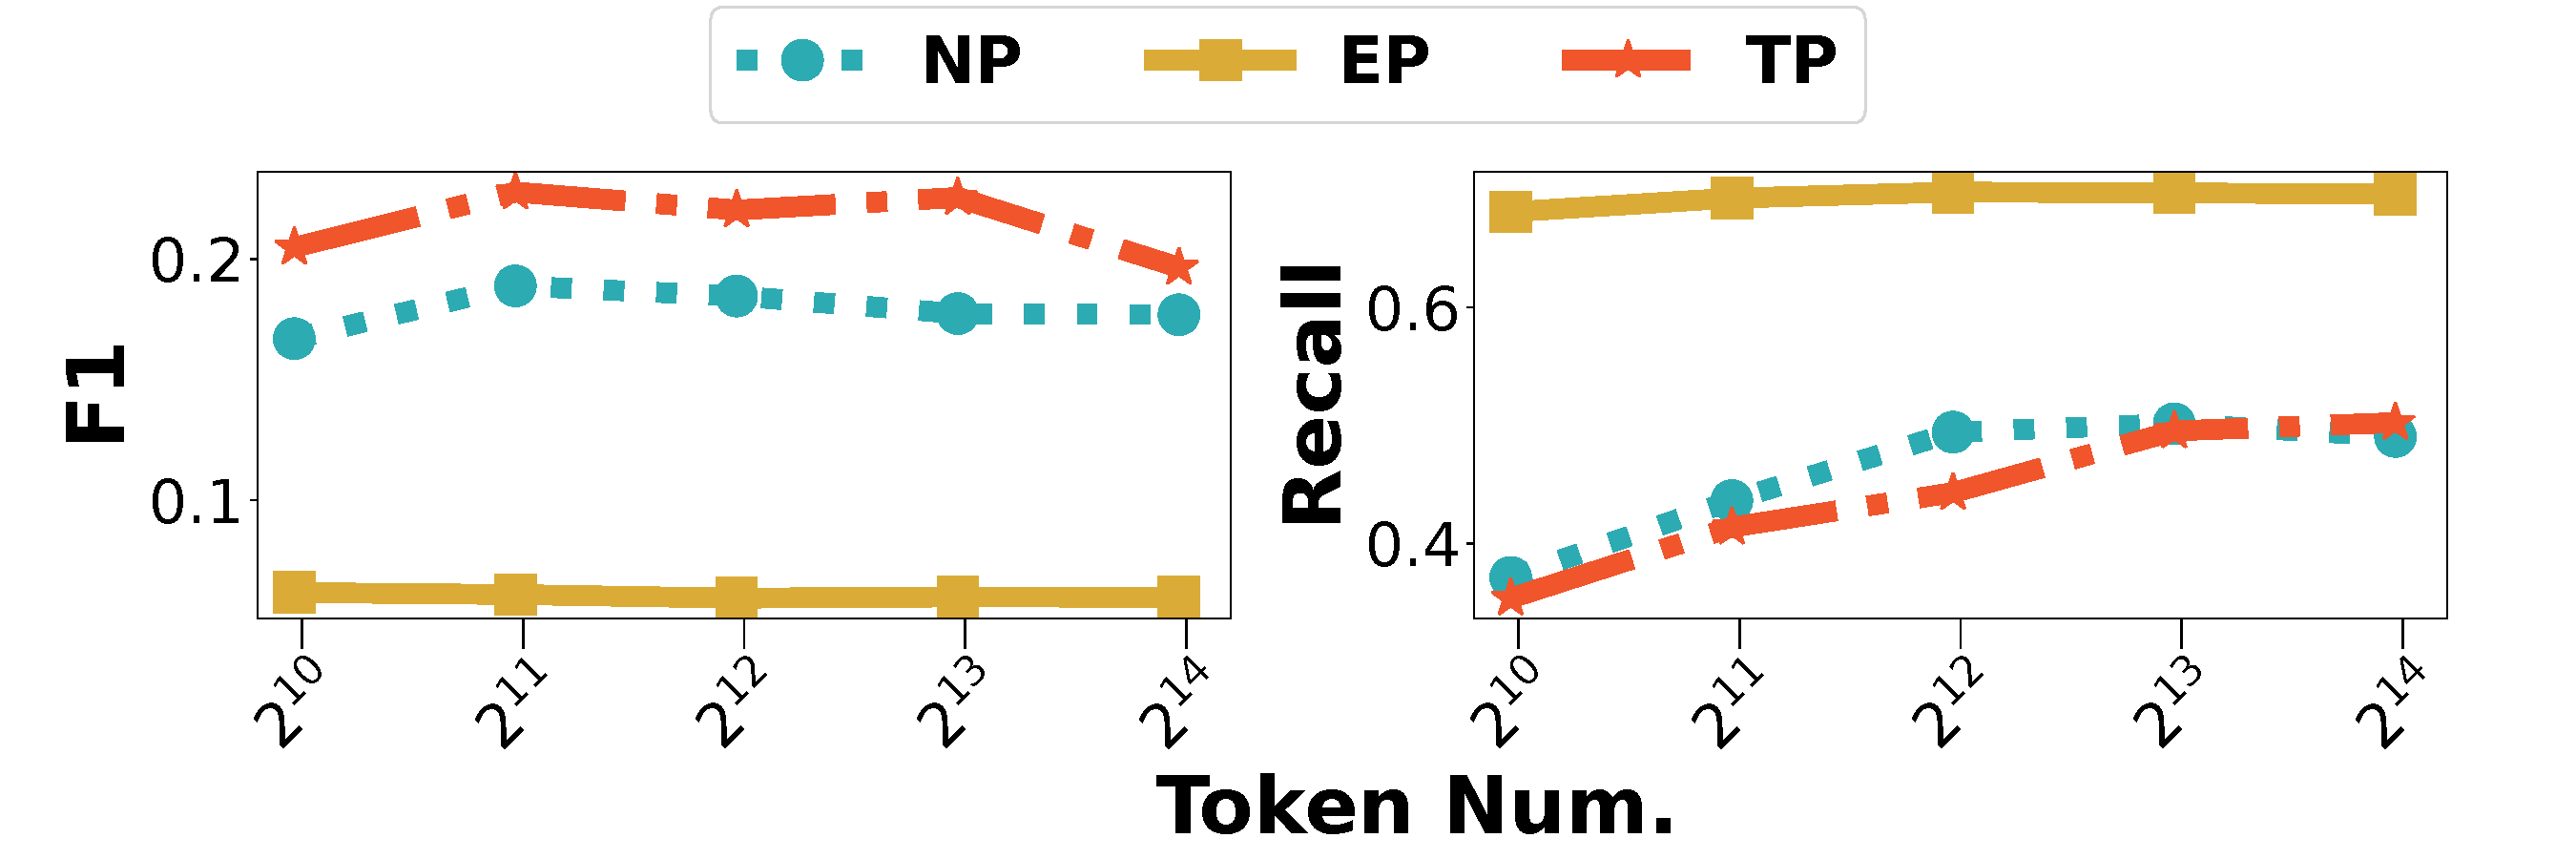
\includegraphics[width=0.48\textwidth]{figures/SE/LLMModel.pdf}
    \vspace{-25pt}
    \caption{Recall, F1 Score w.r.t. Token Cost in SAE-LLMs} 
    \label{fig:SE-LLM-Token}
    \vspace{-10pt}
\end{figure}
\end{comment}

\begin{figure*}[t]
    \centering
    \begin{minipage}[b]{0.3\textwidth}
        \centering
        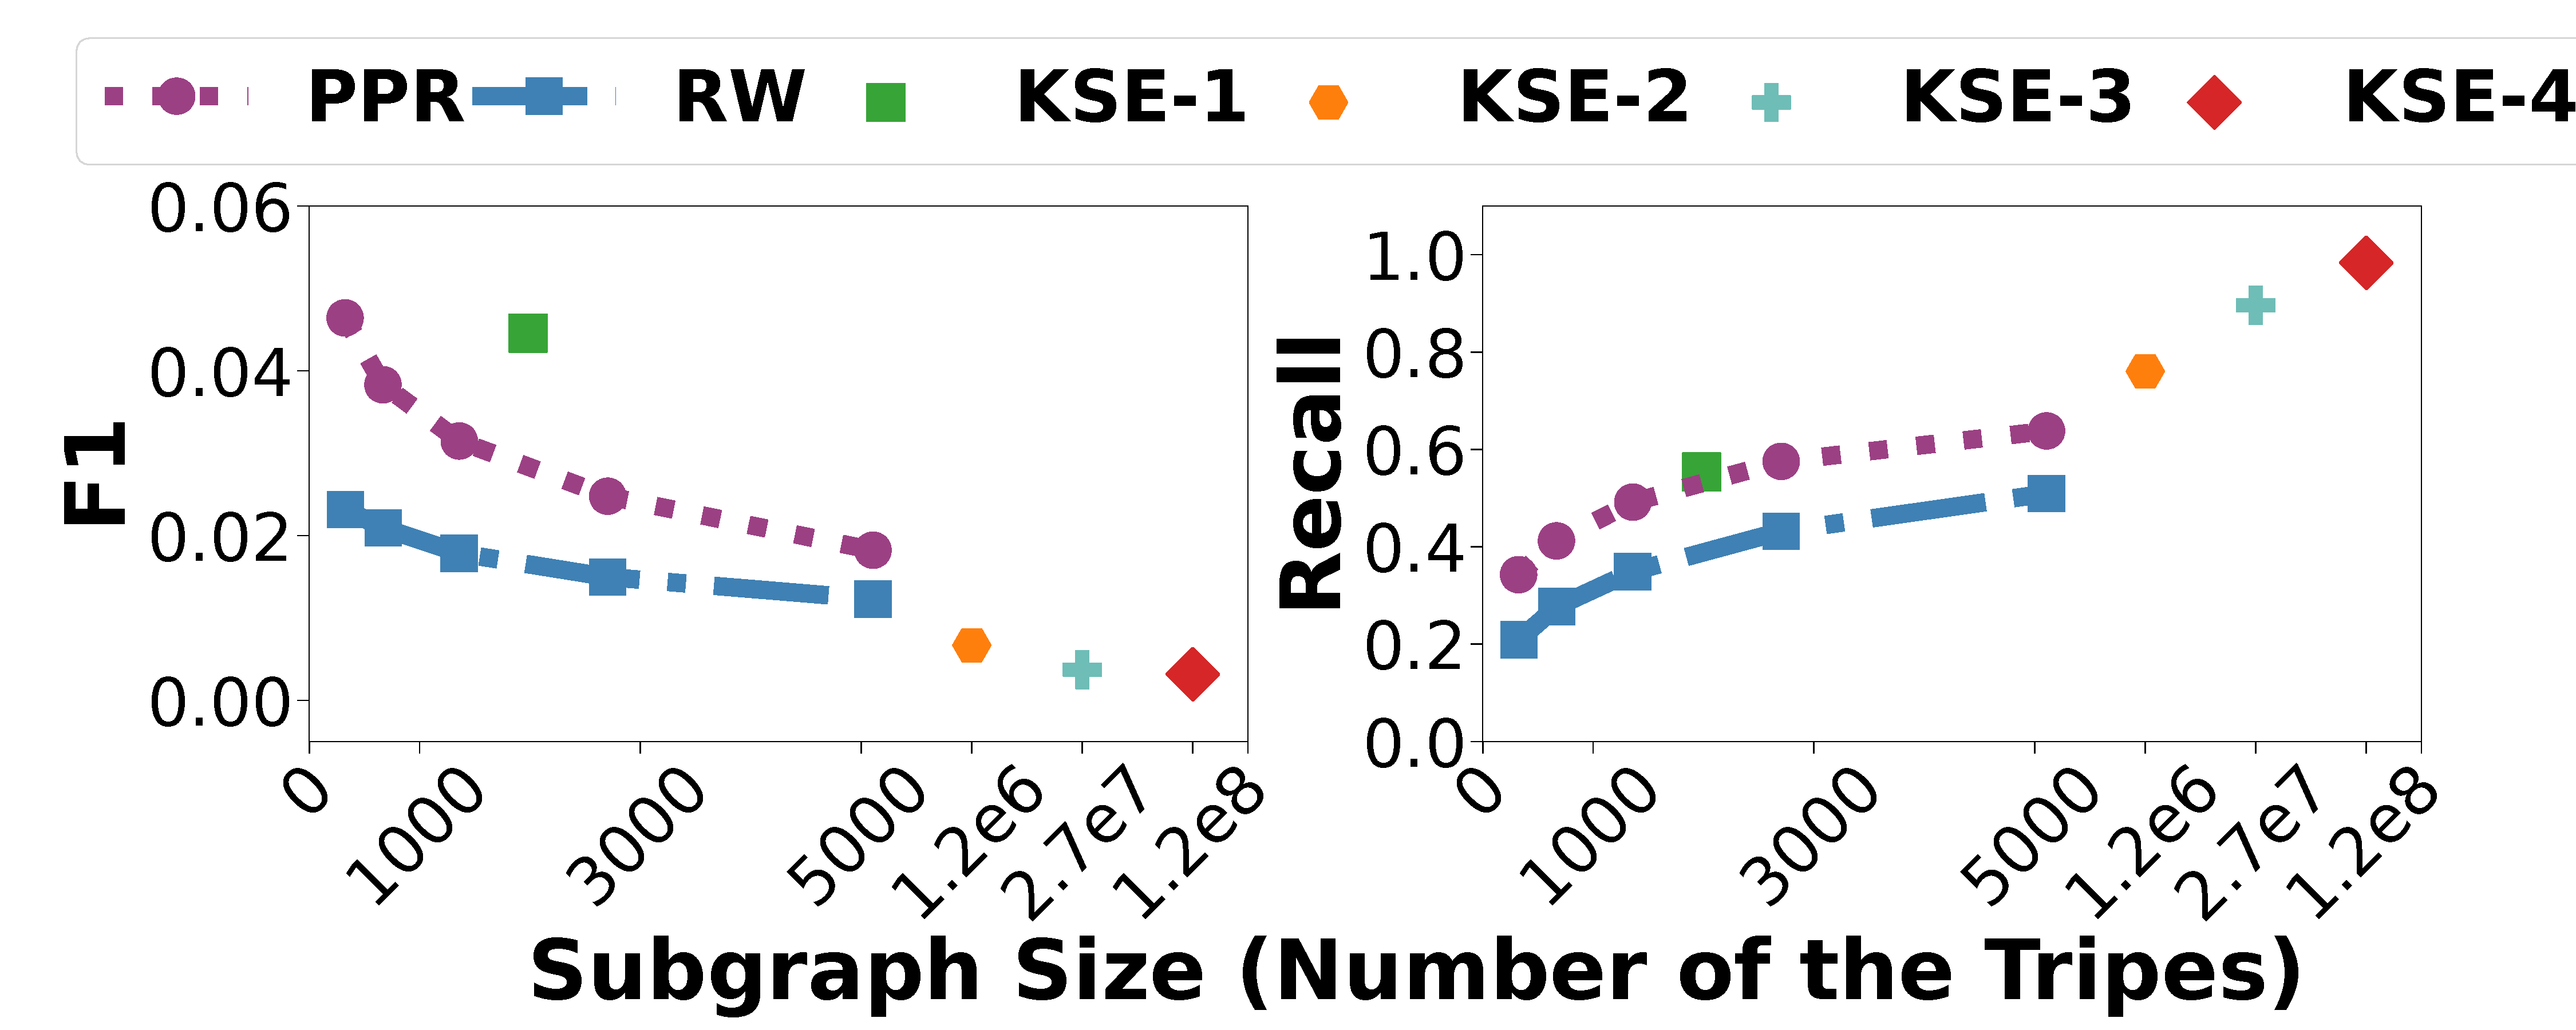
\includegraphics[width=\textwidth]{figures/SE/StructModel.pdf}
        \vspace{-20pt}
        %\caption{\small Recall, F1 Score w.r.t. Subgraph Size in SBE Methods}
        \caption{\small Results w.r.t. Subgraph Size (SBE)}
        %\vspace{-10pt}
        \label{fig:SE-structmodel}
    \end{minipage}%
    \hspace{0.01\textwidth}
    \begin{minipage}[b]{0.3\textwidth} 
        \centering
        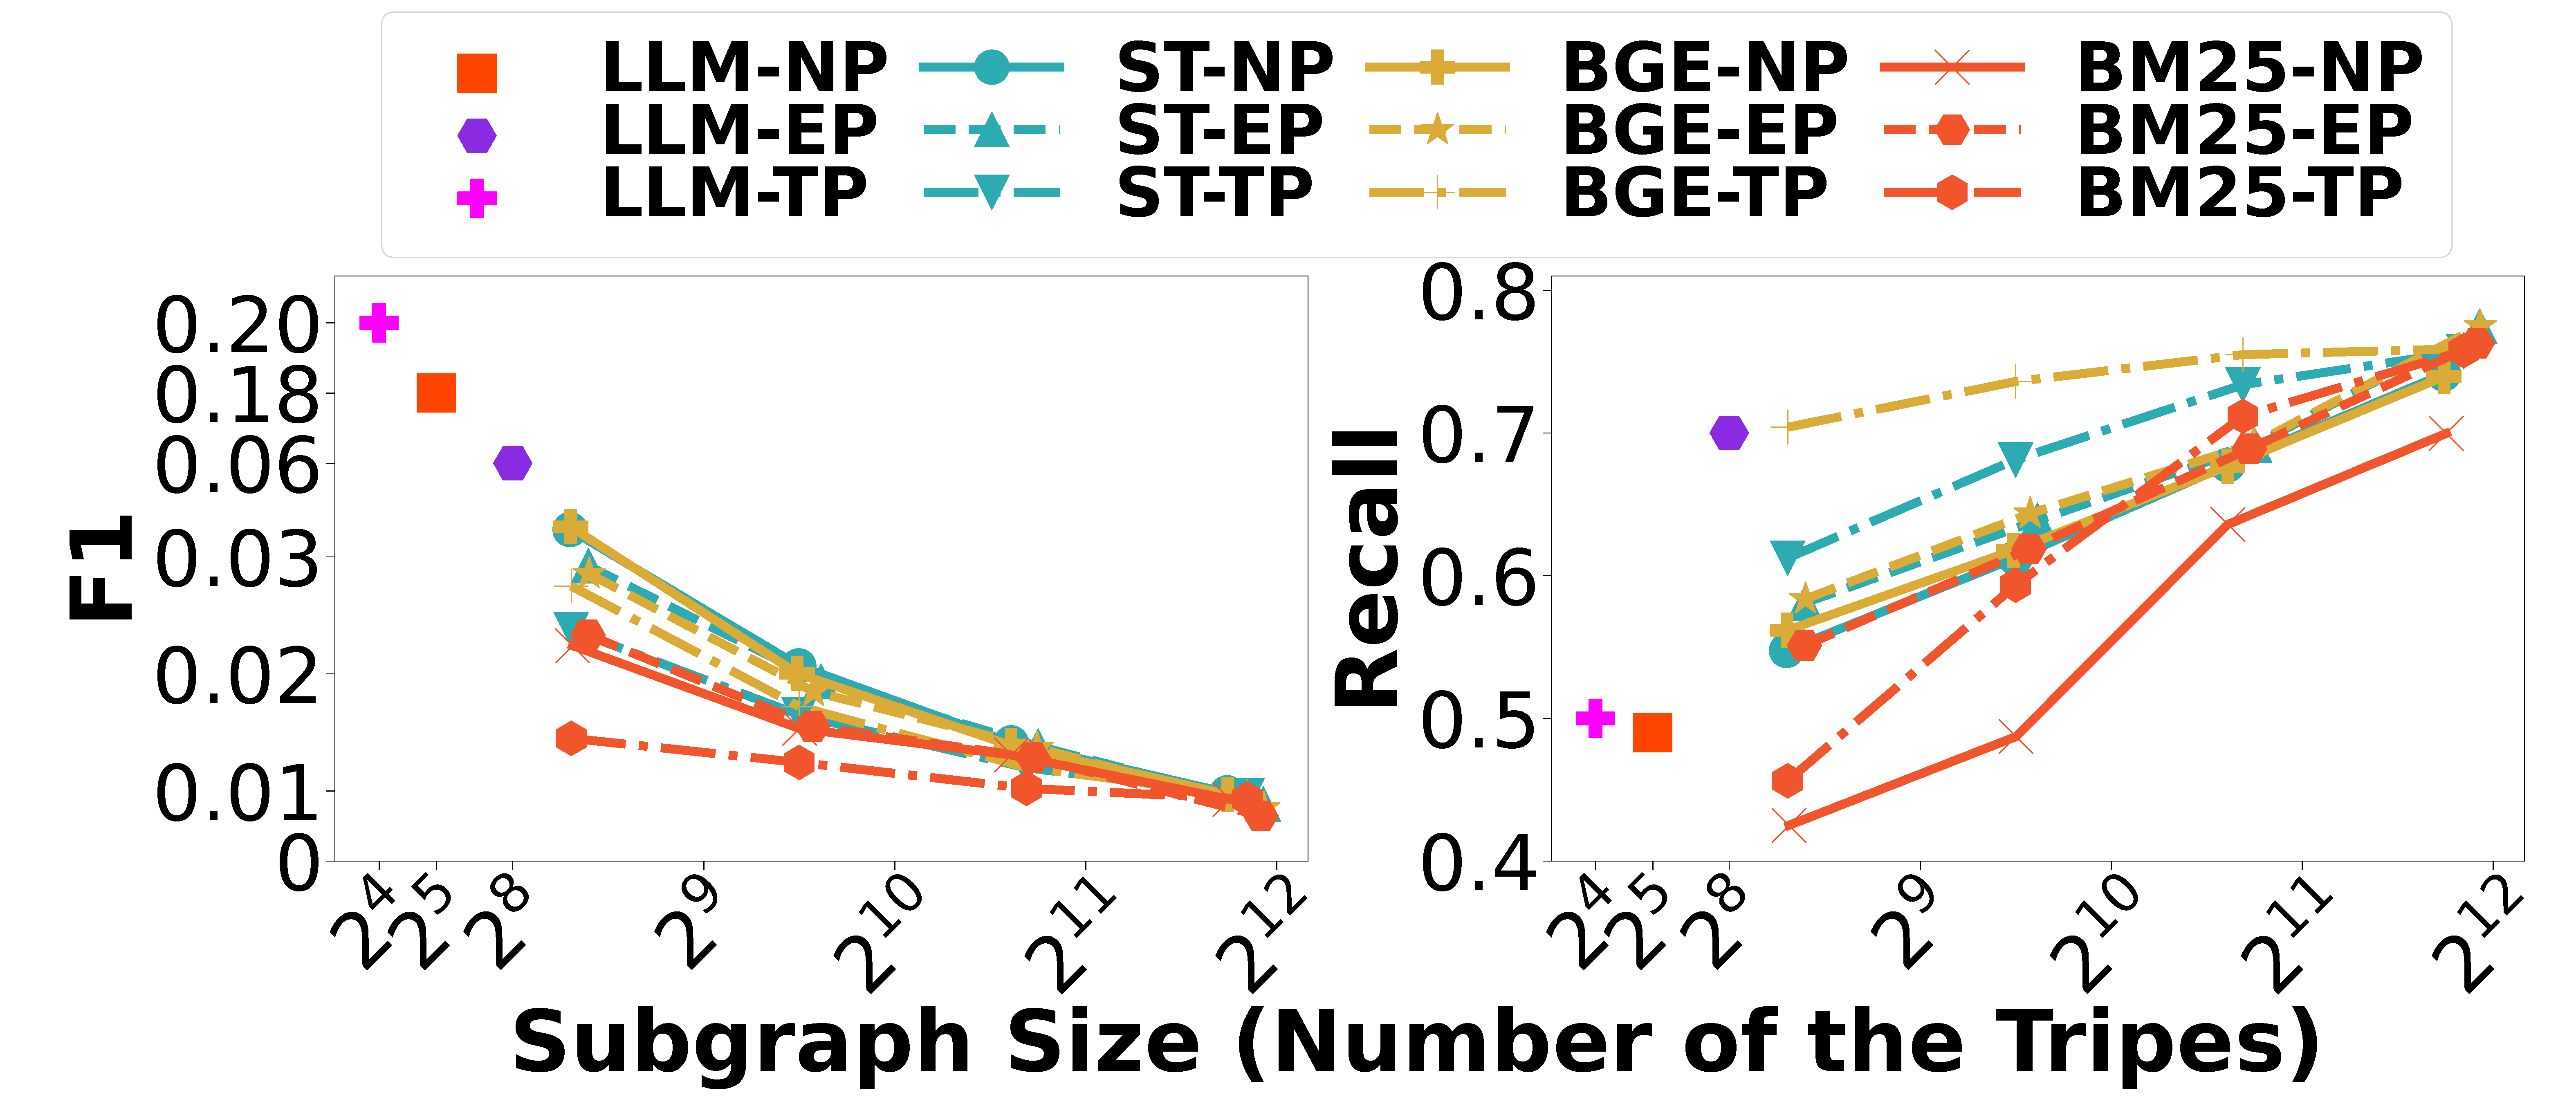
\includegraphics[width=\textwidth]{figures/SE/SmallModel.pdf}
        \vspace{-20pt}
        %\caption{\small Recall, F1 Score w.r.t. Subgraph Size in SAE Methods}
        \caption{\small Results w.r.t. Subgraph Size (SAE)}
        %\vspace{-10pt}
        \label{fig:se-smallmodel}
    \end{minipage}%
    \hspace{0.01\textwidth}
    \begin{minipage}[b]{0.35\textwidth} 
        \centering
        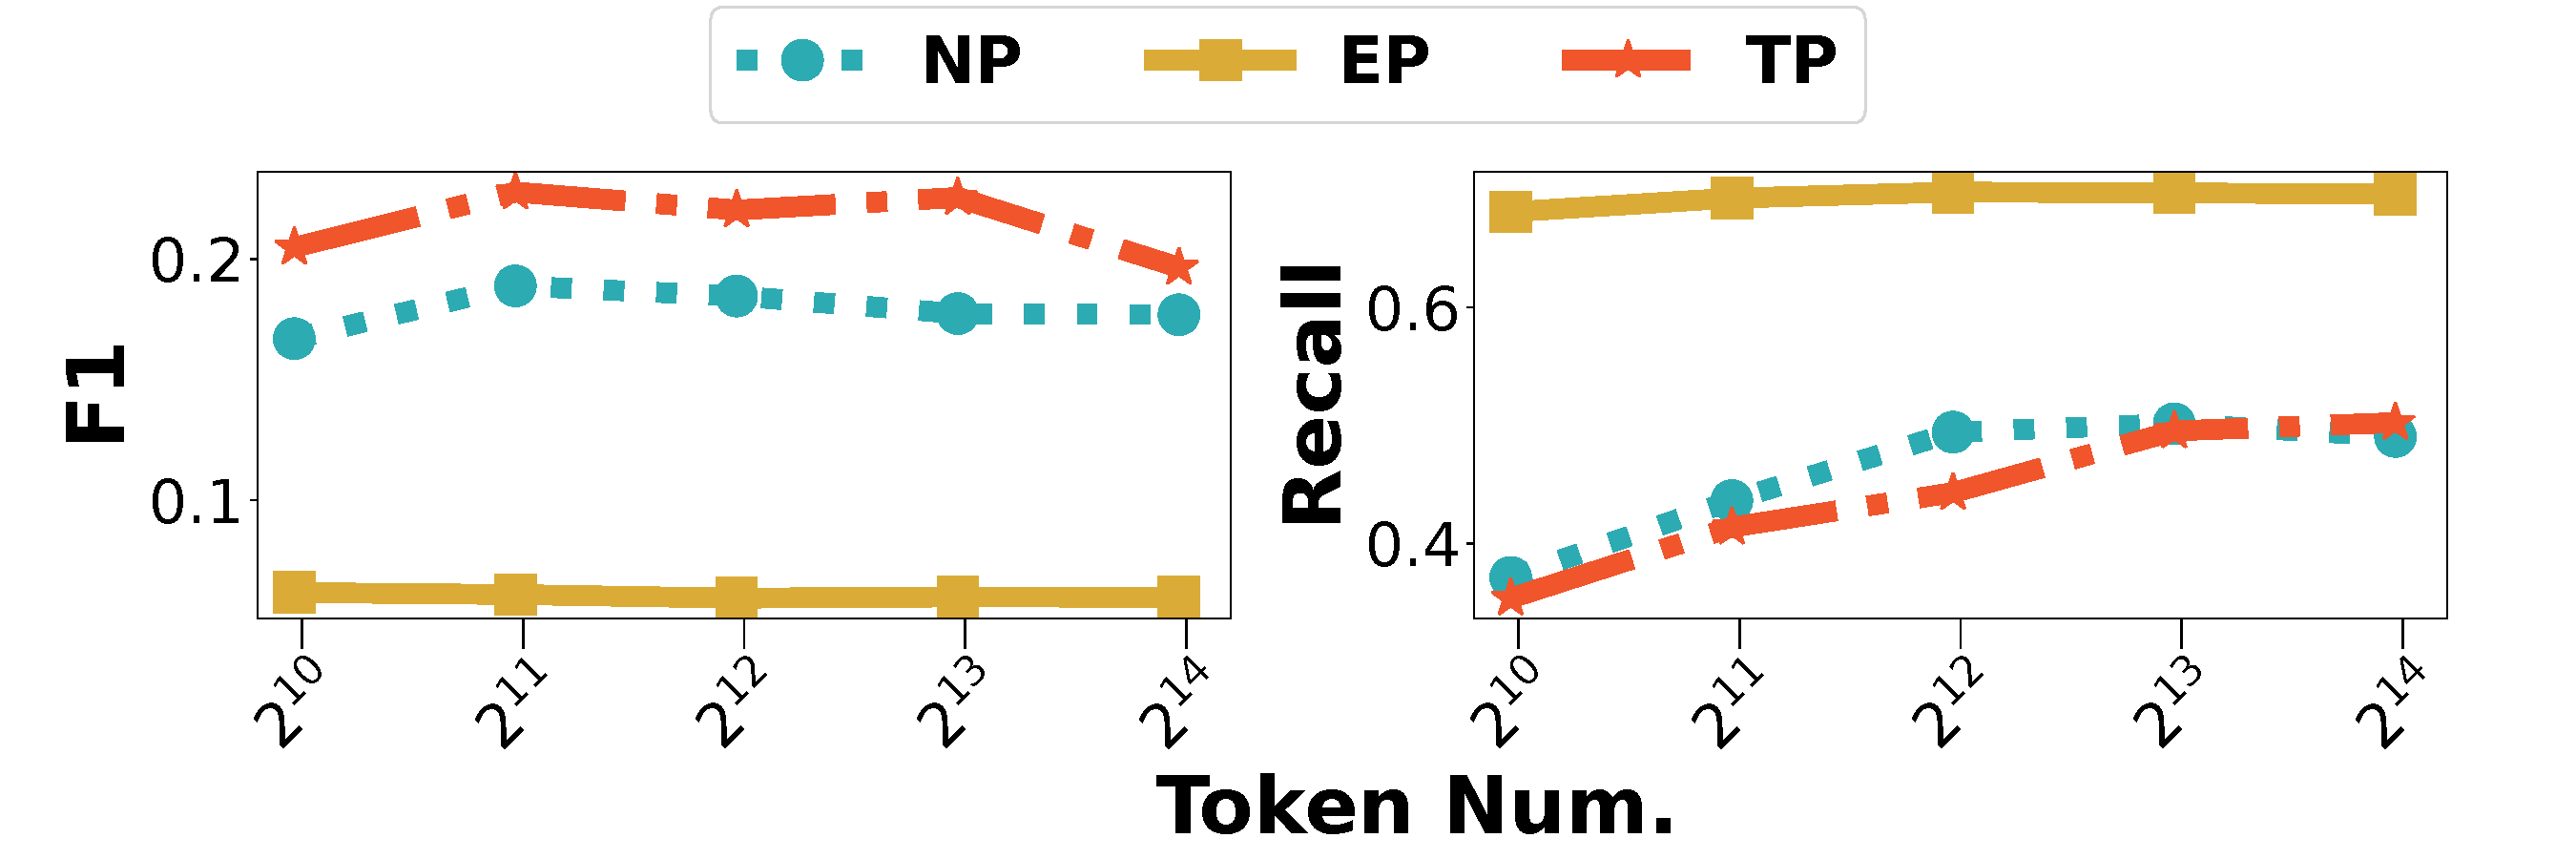
\includegraphics[width=\textwidth]{figures/SE/LLMModel.pdf}
        \vspace{-20pt}
        %\caption{\small Recall, F1 Score w.r.t. Token Cost in SAE-LLMs}
        \caption{\small Results w.r.t. Token Cost (SAE-LLMs)}
        %\vspace{-10pt}
        \label{fig:SE-LLM-Token}
    \end{minipage}%
    %\vspace{-10pt}
\end{figure*}








\subsection{Evaluation of GraphRAG Instances}
\label{exp:instance}
We first present the results of all GraphRAG instances across various metrics and analyze key observations.\footnote{We supplement the evaluation with a case study comparing representative reasoning paths and answers (see technical report B.12).}


%Subsequently, we summarize and highlight the most important findings.


{\it \underline{a) Reasoning Performance.}} 
As shown in Figure~\ref{fig:Instance}, the reasoning performance of different GraphRAG instances across four datasets follows a consistent trend. With the increase in reasoning model size and capabilities (i.e., from 7B LLMs to 72B LLMs), all instances show significant performance improvements. Next, we analyze the instances according to the groups defined in Table~\ref{tab:flat_table}.




\uwave{{\it a).1 Structural Methods on Both Modules (Group (I)).}} 
Instance \\ No.1 of Group (I) exhibits the worst overall performance.
For example, its Hits@1 is only 0.49 (WebQSP with Qwen2-7B), while  most other instances are close to or exceed 0.6. 
This indicates that structure-based methods alone yield baseline solutions, necessitating semantic models for further improvement.
Notably, Instance No.1 outperforms certain semantically augmented instances on specific datasets, such as No.6, No.8, and No.14 (CWQ with Llama3.3-70B). It shows that while semantic augmented methods generally perform better, exceptions depend on query complexity, domain, and integration of semantic models, as discussed later.



\uwave{{\it a).2 Semantic Augmentation on Both Modules (Group (II)).}} 
%In Group (II), the first key observation is that 
In \\ Group (II), instances using EEMs for subgraph-extraction (e.g., No.2, 3, 6, 7) consistently outperform those using LLMs (e.g., No.4, 5, 8, 9) across GrailQA, and all reasoning models. 
This indicates that LLMs are unsuitable for subgraph-extraction when both modules are semantically augmented, as they may overly prune graph information, losing critical intermediate information in the reasoning paths, a limitation seen in instances like GCR~\cite{GCR}, which compromises stability and practicality.

Also, Instances No.2 and 3 in Group (II) achieve the best overall performance, consistently ranking in the top-3 in all reasoning models (WebQSP). 
This highlights the effectiveness of combining EEMs for subgraph-extraction with OSAR for path-retrieval, a strategy yet unexplored by existing methods like GSR~\cite{LessIsMore}, which pairs EEMs with structure-based path-retrieval.
Notably, among Group (II) instances using EEMs for subgraph-extraction (i.e., No.2, 3, 6, 7), Instance No.6 performs the worst. For example, its performance is similar to that of Instance No.1, which uses only structure-based methods (CWQ with all reasoning models). 
This suggests that ISAR pairs better with LLMs than EEMs, as EEMs' weaker semantics can yield noisy scores on long paths and small score gaps, making pruning unreliable. 
One way to improve ISAR-EEMs is to enhance the EEMs themselves, for example, through customization or fine-tuning for specific domains or graphs. In addition, we propose two complementary strategies: {\bf triple-level scoring}, which evaluates only the newly added step at each expansion to reduce error accumulation, and {\bf dynamic pruning}, which adjusts the number of retained paths based on score distribution, helping preserve good candidates when scores are close.\footnote{Detailed discussion and results are available in our technical report B.8.}


\uwave{\textit{a).3 Semantic Augmentation on one Module (Group (III)\&(IV)).}}
\\ We observe that the performance of instances in Group IV (i.e., Instances No.12-15) generally surpasses that of Group III (i.e., Instances No.10, 11).
This suggests that if only one module is semantically augmented, prioritizing the path-retrieval module over the subgraph-extraction module is more effective.  
Using structure-based methods for subgraph extraction remains efficient and sufficient, unlike existing instances such as RoG~\cite{RoG} and GCR~\cite{GCR}, which use LLMs (Llama-2-7b, Llama-3.1-8b) for subgraph-extraction and encounter performance and efficiency bottlenecks.
Additionally, Group (II) instances do not consistently outperform Groups (III) and (IV), implying that semantically augmenting both modules is unnecessary in resource-limited contexts.
Moreover, as shown in Figure~\ref{fig:metaqa}, results on MetaQA align with findings from Freebase-based datasets. The small scale and single-domain nature of the graph lead to uniformly high scores across all instances. Notably, Instance No.14 (ISAR-EEMs) performs comparably to or slightly better than Instance No.15 (ISAR-LLMs), suggesting that EEMs can be a viable and more efficient alternative to LLMs in such settings. 


%, particularly in resource-constrained scenarios.



{\it \underline{b) Runtime.}} Figure~\ref{fig:Instance-time} shows the average runtime of different GraphRAG instances for subgraph-extraction and path-retrieval modules on a single query.
%\footnote{Under our reasoning path settings, the average reasoning time for each model is 0.25s for Qwen2-7B, 0.31s for Glm4-9B, 2.12s for Qwen2-72B, 1.49s for Llama3.3-70B.}. % using vLLM~\cite{vLLM}.}
A key observation is that subgraph-extraction is the primary bottleneck in GraphRAG runtime of all instances. 
For example, Instance No.1, using structure-based methods, requires approximately 70 seconds for subgraph-extraction (i.e., PPR algorithm) but less than 0.1 seconds for path-retrieval.
Since subgraph-extraction is a crucial but time-intensive step in the GraphRAG workflow, it poses significant challenges for the practical development of GraphRAG systems on large-scale graphs like Freebase.
Unfortunately, most existing instances, such as KELP~\cite{ref:kelp}, ToG~\cite{ToG}, and DoG~\cite{DoG}, overlook the efficiency of this process. 
%In Section X, we provide a more in-depth analysis and discussion of this challenge.

Additionally, in the path-retrieval, methods using LLMs (especially under ISAR) exhibit  longer runtimes compared to those using EEMs.
For example, Instance No.12 (OSAR-EEMs) and No.14 (ISAR-EEMs) complete path-retrieval in under 1.15 seconds and 0.19 seconds, respectively, while Instance No.13 (OSAR-LLMs) and No.15 (ISAR-LLMs) take 66.64 seconds and 122.43 seconds, respectively, on GrailQA. 
This shows that using the ISAR-LLMs methods in the path-retrieval  may result in 
unacceptably low query efficiency.

%This indicates that incorporating LLMs or ISAR methods in the path-retrieval module leads to substantially longer and less feasible overall runtime~\footnote{In the retrieval phase, for a fair comparison, we deployed all models based on the transformers~\cite{transformers} library. The runtime of LLMs can be alleviated by employing efficient LLM inference frameworks,  such as vLLM~\cite{vLLM}.}.%TensorRT-LLM, DeepSpeed-MII,

%instances utilizing LLMs exhibit significantly longer running times compared to those using EEMs; The running time of the interactive semantic-augmented retrieval (ISAR) method is generally longer than that of the one-way semantic-augmented retrieval (OSAR) method. 

{\it \underline{c) Cost.}} Figures~\ref{fig:Instance-token} and~\ref{fig:GPU} show the average token overhead (EEMs and LLMs) and peak GPU memory usage (average of four datasets) across GraphRAG instances. 
Instances mixing EEMs and LLMs (e.g., No.3, 4, 7, 8) incur higher token costs than those using the same model type (e.g., No.2, 5, 6, 9), with EEM-only setups being the most economical.
%Regarding token overhead, we observe that instances employing different types of semantic models across the two modules (i.e., Instances No.3, No.4, No.7, and No.8), where one module uses EEMs and the other uses LLMs, consume more tokens than instances that use the same type of semantic model in both modules (i.e., Instances No.2, No.5, No.6, and No.9). Thus, utilizing the same type of semantic model in both modules, particularly the more cost-effective EEMs, can reduce token overhead and prove to be more economical.
%For GPU memory usage, instances solely using EEMs have relatively low requirements, typically under 1GB, while those incorporating LLMs require significantly more. Notably, instances using LLMs in both modules (e.g., Instances No.5 and No.9) can peak at up to 80GB of GPU memory. In summary, while semantic augmentation boosts performance, the associated high computational and GPU memory costs present significant challenges for deploying GraphRAG systems, especially with LLMs. 
%These observations highlight the trade-offs in semantic augmentation, stressing the need to optimize the balance between quality and cost.
GPU usage remains low (<1GB) for EEM-only instances but rises sharply for LLM-based ones, peaking at ~80GB when LLMs are used in both modules (e.g., No.5, 9). The results underscore the performance–cost trade-offs of semantic augmentation and the importance of corresponding optimization.
%for optimizing quality and efficiency.

%Optimizing token usage and memory consumption will be essential for more efficient future system designs.



%{\it \underline{d) One-, Two-, and Multi-Hop Queries.}} Figure~\ref{fig:hops} shows the average Hits@1 of GraphRAG instances on one-, two-, and multi-hop query tasks.
%For one-hop queries, Instance No.1, using only structure based methods, performs comparably to instances with semantic augmentation. However, its performance drops significantly for two- and multi-hop queries, highlighting the importance of semantic information in complex reasoning.
%Even the best-performing Instance No.2 achieves Hits@1 of only 0.55 for two-hop tasks and 0.48 for multi-hop tasks, indicating substantial room for enhancing GraphRAG instances in handling complex reasoning tasks.

{\it \underline{d) Analysis by Query Type.}}  
We analyze performance across different query types %based on three criteria: 
by varying reasoning hops, number of answers, and number of query entities. As shown in Figure~\ref{fig:Hop}, performance consistently declines with more reasoning hops, especially for structure-based methods (e.g., Instance No.1), which struggle on multi-hop queries. 
%indicating the greater difficulty of multi-hop queries across all instances.
Figure~\ref{fig:Answer} shows a similar drop from single- to multi-answer queries, where semantic methods are more resilient.
%Structure-based methods (e.g., Instance No.1) perform comparably to semantic-augmented methods on one-hop queries but drop significantly on two- and multi-hop queries. Figure~\ref{fig:Answer} further shows that performance drops notably from single- to multi-answer queries, where semantic-augmented methods are more robust as the number of answers increases. 
Figure~\ref{fig:Entity} shows improved performance with more query entities, likely due to increased chances of retrieving relevant paths—even benefiting structure-only instances like No.1.
%reveals that performance tends to improve with more query entities, likely because additional entities increase the chances of retrieving relevant paths from the graph, benefiting even instances  No.1 that rely solely on structural information. 

{\it \underline{e) Integrating Microsoft GraphRAG.}} To evaluate compatibility with Microsoft GraphRAG, we implement an instance (GRAG-M), which follows its workflows: performing community detection on the graph and precomputing textual summaries for each community. 
On the MetaQA dataset, GRAG-M uses the reasoning paths from Instance 12 (which showed strong performance in our experiments) and provides both the paths and summaries as input to the LLMs.
%The instance is evaluated on MetaQA, a semantically rich dataset well-suited for precomputation. During  generation phase, both the retrieved reasoning paths~\footnote{Paths are from Instance 12 (SBE-PPR + OSAR-EEMs), which showed strong performance in our experiments.} and the summary of the query-related community are provided to the LLMs.
As shown in Figure~\ref{fig:metaqa}, GRAG-M performs well on Qwen2-7B and Glm4-9B. Gains diminish with Qwen2-72B, where the larger model already captures sufficient context, reducing the benefit of precomputed summaries. 
%achieves strong performance across several reasoning models (Qwen2-7B and Glm4-9B). Its improvement narrows on Qwen2-72B, where the larger LLMs may already capture sufficient context, reducing the benefit of the precomputed summaries.  

\begin{comment}

{\it \underline{e) Summary of Key Findings.}}
%\begin{itemize}[leftmargin=15pt]
%    \item 

{\bf Finding 1: GraphRAG Trade-off Structure.} GraphRAG entails multi-aspect trade-offs among quality (Hits@1), efficiency (runtime), and cost (token and GPU usage). This trade-off spans two modules (subgraph-extraction vs. path-retrieval), two method types (structure-based vs. semantic-augmented), and two types of semantic models (EEMs vs. LLMs).

    %\item 
    \textbf{Finding 2: Module-level Trade-offs.} Subgraph-extraction is the main efficiency bottleneck for large-scale graphs. Overuse of semantic augmentation (e.g., using LLMs) in subgraph-extraction can compromise downstream parth-retrieval quality. Targeting semantic augmentation in the path-retrieval module is a more cost-effective strategy to maintain high quality.
    %For quality, due to the sequential dependency between the two modules, excessive semantic augmentation (e.g., using LLMs) in subgraph-extraction may lead to the loss of critical information in path-retrieval, increasing cost and degrading quality. Conversely, applying semantic augmentation solely to the path-retrieval can enhance quality while minimizing cost.
        
    %\item 
    \textbf{Finding 3: Method-level Trade-offs.} Structure-based methods offer higher efficiency and lower cost, but semantic-augmented methods are essential for quality, especially for complex (two- or multi-hop) queries. 
    One-way semantic methods (OSAR) balance quality and efficiency better than interactive methods (ISAR).
    %Among semantic-augmented methods, one-way methods (OSAR) achieve a better balance between quality and efficiency than interactive methods (ISAR), with comparable cost. 

    %\item 
    \textbf{Finding 4: Model-level Trade-offs.} 
    EEMs are more cost effective in token and GPU usage, while LLMs provide better quality, particularly for interactive methods (ISAR). A balanced approach includes applying LLM-based augmentation in path-retrieval or EEM-based augmentation in both modules.
    %To balance quality and cost, either apply LLM-based semantic augmentation solely to the path-retrieval module or use EEM-based semantic augmentation in both modules.

    %\item 
    \textbf{Finding 5: A Promising yet Underexplored Strategy.} Based on the multi-aspect trade-off analysis, the most effective approach for GraphRAG would be the one that combines structure-based methods for subgraph-extraction with OSAR for path-retrieval. Despite its potential, this strategy remains underexplored in existing works. Also, it opens up opportunities for further optimizations for handling complex queries and enhancing overall efficiency.
%\end{itemize}
\end{comment}

%\vspace{-11pt}
\subsection{Evaluation of {\PreRetrieval} Module}
\label{exp:PreRetrieval}

%\vspace{-5pt}
%\textbf{PPR Consistently Delivers the Best Quality in SBE Solutions.}
{\bf Structure-Based Extraction (SBE).}  
Figure~\ref{fig:SE-structmodel}
%\footnote{Due to space limitations, Figures 7-11 report the average results across the 4 datasets.} 
shows the variation in F1 score and Recall for the three SBE methods (RW, PPR, and KSE) as the extracted subgraph size changes. The F1 score for all methods decreases as the subgraph size increases, while their Recall consistently improves. Across all subgraph sizes, PPR consistently outperforms RW in both F1 score and Recall, demonstrating the superior effectiveness of PPR over RW. Additionally, RW struggles to achieve a Recall above 60\%, rendering it nearly unusable in GraphRAG.  
Moreover, PPR offers greater flexibility compared to KSE, enabling precise control over subgraph size through hyperparameters. In contrast, KSE relies on hierarchical extraction, which lacks such flexibility.\footnote{Many prior studies {\cite{RoG,GCR,LessIsMore,StructGPT}} first apply KSE to extract 2-hop or 4-hop subgraphs, followed by PPR to distill them into smaller, query-relevant subgraphs.}
These advantages establish PPR as the current optimal solution for SBE. 
As Table~\ref{tab:pprtime} demonstrates, PPR's computational costs become prohibitive for large graphs. 
%Section~\ref{subsec:eeSE} explores potential optimizations.
%{\color{blue} However, as shown in Table~\ref{tab:pprtime}, PPR encounters significant computational bottlenecks on large graphs, with runtime becoming prohibitively slow. We explore optimization directions to address this issue in Section~\ref{subsec:eeSE}. {\bf (For R1: W1(D1.a,b))}}


%Although some approximate top-$k$ PPR methods from the database community (as shown in Table~\ref{tab: PPR-Acceleration}) can optimize computation time, they lead to a substantial drop in Recall, which negatively impacts subsequent path-retrieval modules. This trade-off underscores a critical research direction for the community: developing methods that effectively balance computational efficiency and subgraph quality.
%For example, future studies could explore pre-extracting possible query subgraphs {\cite{SubgraphRAG,GraphRAG}} or developing efficient and quality-assured SBE methods, such as approximate PPR {\cite{Fora,Topppr,Fora+}}  and distributed PPR {\cite{kPAR,DistPPR,GPA}}.

%{\color{red} Appendix~\ref{appendix:Addtion results} shown the variation curve of computational overhead with subgraph size of SBE, the time of PPR is constant at around 70s, while the time overhead of KSE and RW increases with the size of the subgraph. }

%TP performs best at smaller subgraph scales. However, as the subgraph size increases, the effectiveness of EP, TP and NP based on EEMs converges with that of PPR. Ultimately, EP slightly outperforms TP, which is comparable to PPR, while TP marginally surpasses NP. Across all pruning methods and subgraph scales, Re-Ranker consistently outperforms ST, and ST consistently surpasses BM25.
%It is noteworthy that LLM retrieves significantly smaller subgraphs, reducing the size by approximately eightfold or more. While this compression may lead to diminished downstream path-retrieval quality, as highlighted in \textbf{Finding 2}. Furthermore, the evaluation demonstrates that EP on LLM outperforms both NP and TP, achieving a remarkable Recall improvement of nearly 0.2, underscoring its superior effectiveness.

%\textbf{EP and TP Achieve Highest Quality in Large and Small Subgraph Scales respectively, while Re-Ranker Outperforms ST and BM25 Across All Scales in SAE Solutions with EEMs.} 
% \input{./tables/DifferentPPR.tex}

\begin{figure}[t]
    \centering
    \begin{minipage}[b]{0.24\textwidth}
        \centering
    
        \captionof{table}{\small PPR Runtime  w.r.t. Graph Size}  % w.r.t. with respect to 关键修改
        \vspace{-5pt}
        \label{tab:pprtime}
        \resizebox{\linewidth}{!}{%
            \begin{tabular}{l|l|l}
            \toprule
            \textbf{Nodes} & \textbf{Ave. Edges} & \textbf{Ave. Time (s)} \\
            \midrule
            100000    & 431414.5    & 0.58 \\
            1000000   & 5567538.1   & 1.37 \\
            10000000  & 48865879.2  & 11.5 \\
            100176641 & 298458255   & 75.29 \\
            \bottomrule
            \end{tabular}
        }
        \vspace{-5pt}
    \end{minipage}%
    \hspace{0.01\textwidth}
    \begin{minipage}[b]{0.21\textwidth} 
        \centering
        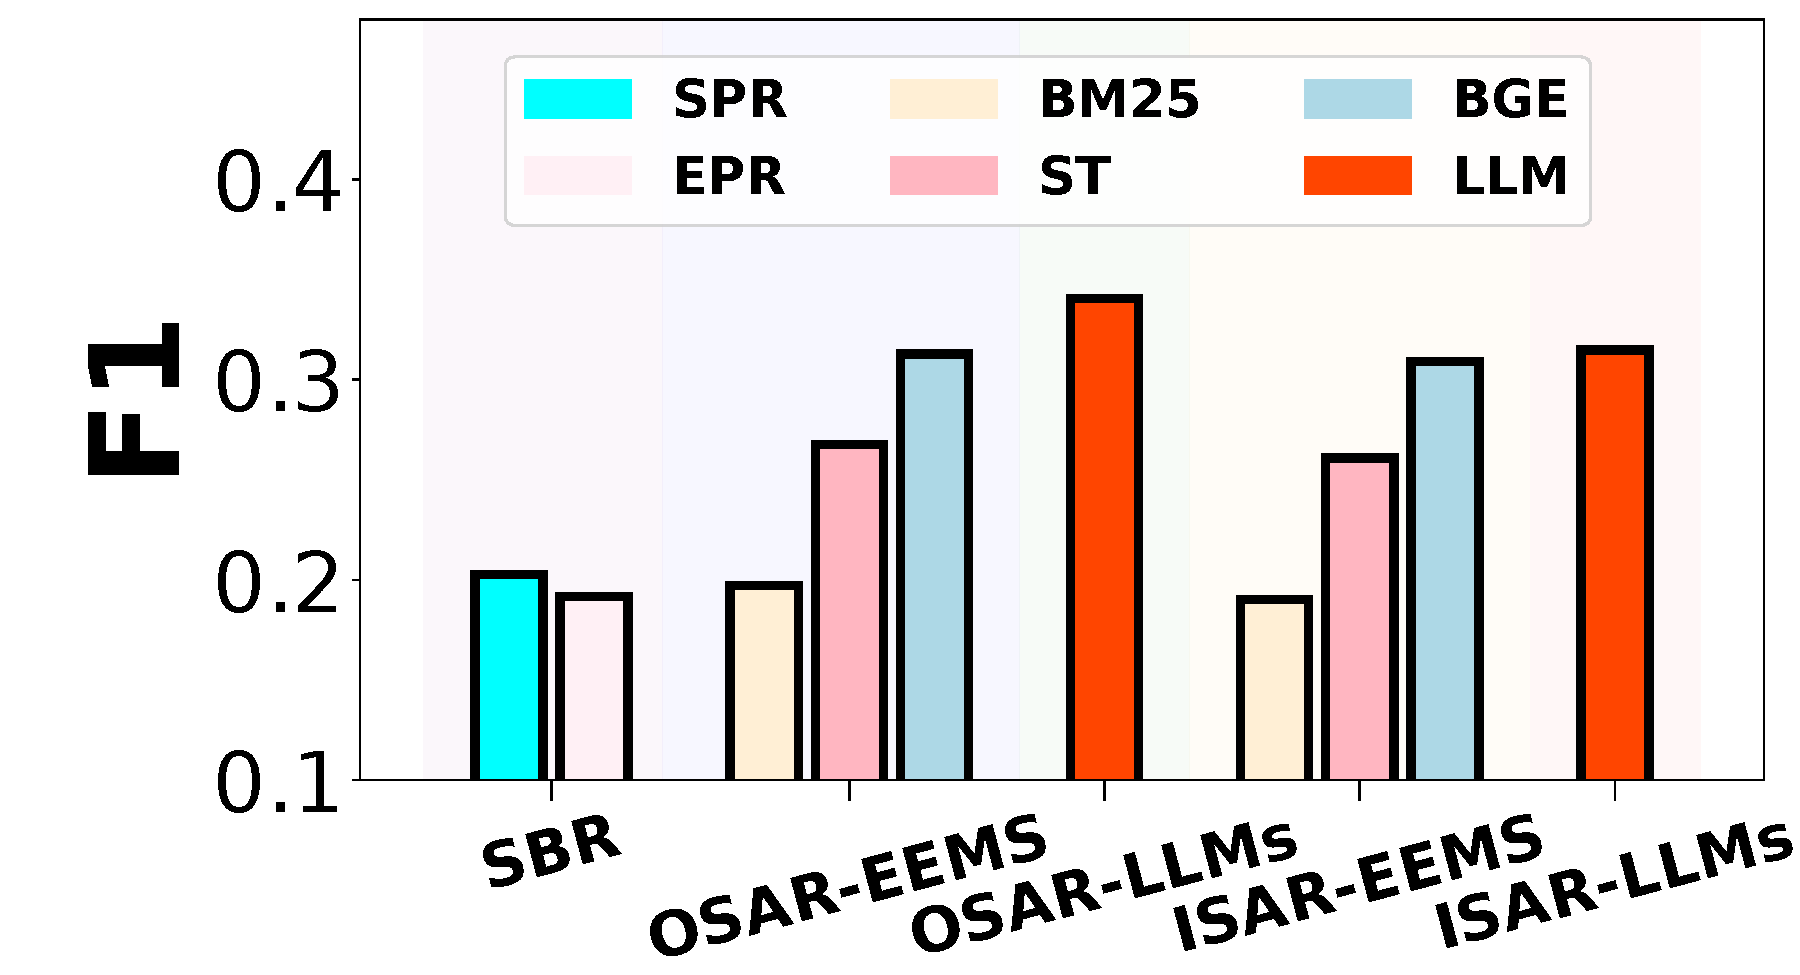
\includegraphics[width=\textwidth]{figures/PR/PR-F1-32.pdf}
        \vspace{-21pt}
        \caption{\small F1 Score of Methods in Path-Retrieval Module}
        \vspace{-5pt}
        \label{fig:PR-LLM}
    \end{minipage}%
    %\vspace{-10pt}
\end{figure}

{\bf Semantic-Augmented Extraction (SAE).}
Figure~\ref{fig:se-smallmodel} shows the Recall and F1 score of different semantic model combinations with three subgraph pruning strategies  under the SAE methods, as the subgraph size varies. %, with PPR as the baseline. 
Among the three semantic models, the BGE and ST significantly surpass BM25 across all pruning strategies and subgraph scales. BGE is slightly better in quality, while ST is even better in efficiency,  as discussed later. 
Considering the trade-off between quality and efficiency, we propose to use ST as the representative EEMs.
For the three pruning strategies, TP exhibits the best quality at smaller subgraph scales, while NP performs the worst. However, as subgraph size increases, the F1 score and Recall of EP, TP, and NP converge. Ultimately, EP slightly outperforms TP, while TP marginally surpasses NP.
Thus, TP is recommended when the size of the extracted subgraph is small; otherwise, EP.
%LLM-based methods produce significantly smaller subgraphs, achieving an approximate eightfold reduction in size or more. This compression can lead to impact downstream path-retrieval quality (as discussed in \textbf{Finding 2}). EP on LLM demonstrates superior performance compared to NP and TP. Notabtly, EP achieves a Recall improvement of nearly 0.2, highlighting its effectiveness in subgraph pruning for LLMs. 

%\textbf{EP Strikes the Optimal Balance of Quality and Token Efficiency in SAE Solutions with LLMs.}

Due to the inherent uncertainty in LLM outputs, SAE-LLMs methods often struggle to control the size of subgraphs extracted, typically producing smaller subgraphs that can reduce path-retrieval quality (see \textbf{Finding 2}).  
Figure~\ref{fig:se-smallmodel} shows the F1 score and Recall for subgraphs generated using SAE-LLMs under three pruning strategies, plotted against the average subgraph size. 
Among the three pruning strategies, EP outperforms NP and TP for SAE-LLMs.
Figure~\ref{fig:SE-LLM-Token} further shows the trends in F1 score and Recall as the number of tokens input into the LLMs varies for NP, TP and EP. Recall for NP consistently surpasses that of both TP and EP, maintaining a gap of around 0.2. Although EP underperforms in terms of F1 score due to the larger subgraphs it extracts, the relatively low Recall of NP and EP may diminish their effectiveness in path-retrieval. As the number of tokens increases, Recall for NP and TP initially rises, then declines, while EP remains nearly constant, indicating that EP achieves more effective subgraph extraction at a lower token cost for the SAE-LLMs methods.
The efficiency of SAE methods is related to the semantic models used. Runtime is influenced by factors such as model parameters, algorithmic complexity, and data volume. In general, the runtime for processing a graph component follows this order: LLMs > BGE > ST > BM25, as shown in Figure~\ref{fig:PR-cost}.




\begin{table}[h]

    \centering  
    \caption{\small Results of Hybrid ISAR Combining EEMs and LLMs}
    \vspace{-10pt}
    \label{tab:ISAR_h}  
    \resizebox{0.46\textwidth}{!}{%  
    \begin{tabular}{l|l|l|l|l}  
        \toprule  
        \textbf{Method}
        & \textbf{CWQ}  & \textbf{WebQSP} & \textbf{GrailQA} & \textbf{WebQuestion} \\ \midrule  
                \textbf{SBE+ISAR-EEMs}                         & 0.183         & 0.157           & 0.395             & 0.16                \\
        %\textbf{SBE+ISAR-EEMs (LLMs-ES)} & 0.135         & 0.117           & 0.304            & 0.120                \\

        \textbf{SBE+ISAR-EEMs (LLMs-R)}          & \textbf{0.271}         & \textbf{0.219}           & \textbf{0.379}            & \textbf{0.175}                \\
           \midrule  \midrule  
        \textbf{SBE+ISAR-LLMs}                         & 0.249         & 0.264           & 0.371             & 0.249                \\
        \textbf{SBE+ISAR-LLMs (EEMs-PF)}                           & 0.271         & 0.316           & 0.396            & 0.245                \\
        \textbf{SBE+ISAR-LLMs (EEMs-S)}             & \textbf{0.310} & \textbf{0.373}  & \textbf{0.435}   & \textbf{0.276}       \\      
        \bottomrule 
    \end{tabular}  
    } 
    \vspace{-12pt}
\end{table} 

\subsection{Evaluation of {\Retrieval} Module}
\label{exp:Retrieval}

%\textbf{OSAR Demonstrates Superior Performance in SAE Solutions with EEMs, while LLM achieve dominance in path-retrieval quality 

Figure~\ref{fig:PR-LLM} shows the F1 score of different methods in path-retrieval module.
   It shows that OSAR outperforms ISAR in all semantic models. SPR method slightly outperforms EPR and I/OSAR with BM25, but underperforms all I/OSAR solutions with ST, BGE or LLM, which suggests that the use of poorer semantic models to aid enhanced retrieval may lead to a loss of quality.
We further investigate the variation in the F1 score of the path-retrieval module when the number of reasoning paths changes, as shown in Figure~\ref{fig:PR-F1}. Since the number of paths output by LLM is inherently uncertain, methods using LLM are excluded.
It shows that the F1 score of SBR and I/OSAR with BM25 gradually increases with the number of paths, yet their F1 score remains low-level, consistently trailing I/OSAR with BGE and ST by approximately 0.1. The gap widens to 0.2 or more when fewer paths are retrieved. In contrast, the performance of I/OSAR with ST and BGE initially improves and then declines as the number of retained paths increases, with OSAR generally outperforming ISAR. Note that F1 scores may be higher for smaller sets of reasoning paths, as they tend to prioritize precision. A slight decrease in F1 for larger reasoning path sets is not indicative of lower quality but rather reflects the broader scope of the retrieved paths.



Figure~\ref{fig:PR-cost} shows the runtime of different methods in the path-retrieval module (WebQSP). Among the SBR solutions, EPR has the longest runtime due to the large number of paths it retrieves, while SPR reduces computation time by retrieving only a single path for each node. 
The EPR-based OSAR method becomes impractical because its excessive data volume results in prohibitive runtime overhead when used with semantic models. As a result, only SPR is employed in this context.
Among the three semantic models, both BGE and ST demonstrate significant quality improvements over BM25 combined with I/OSAR. BGE achieves marginally higher quality, whereas ST exhibits superior efficiency. 

%\vspace{-5pt}
\begin{figure}[t]
    \centering
    \begin{minipage}{0.23\textwidth}
            \centering
        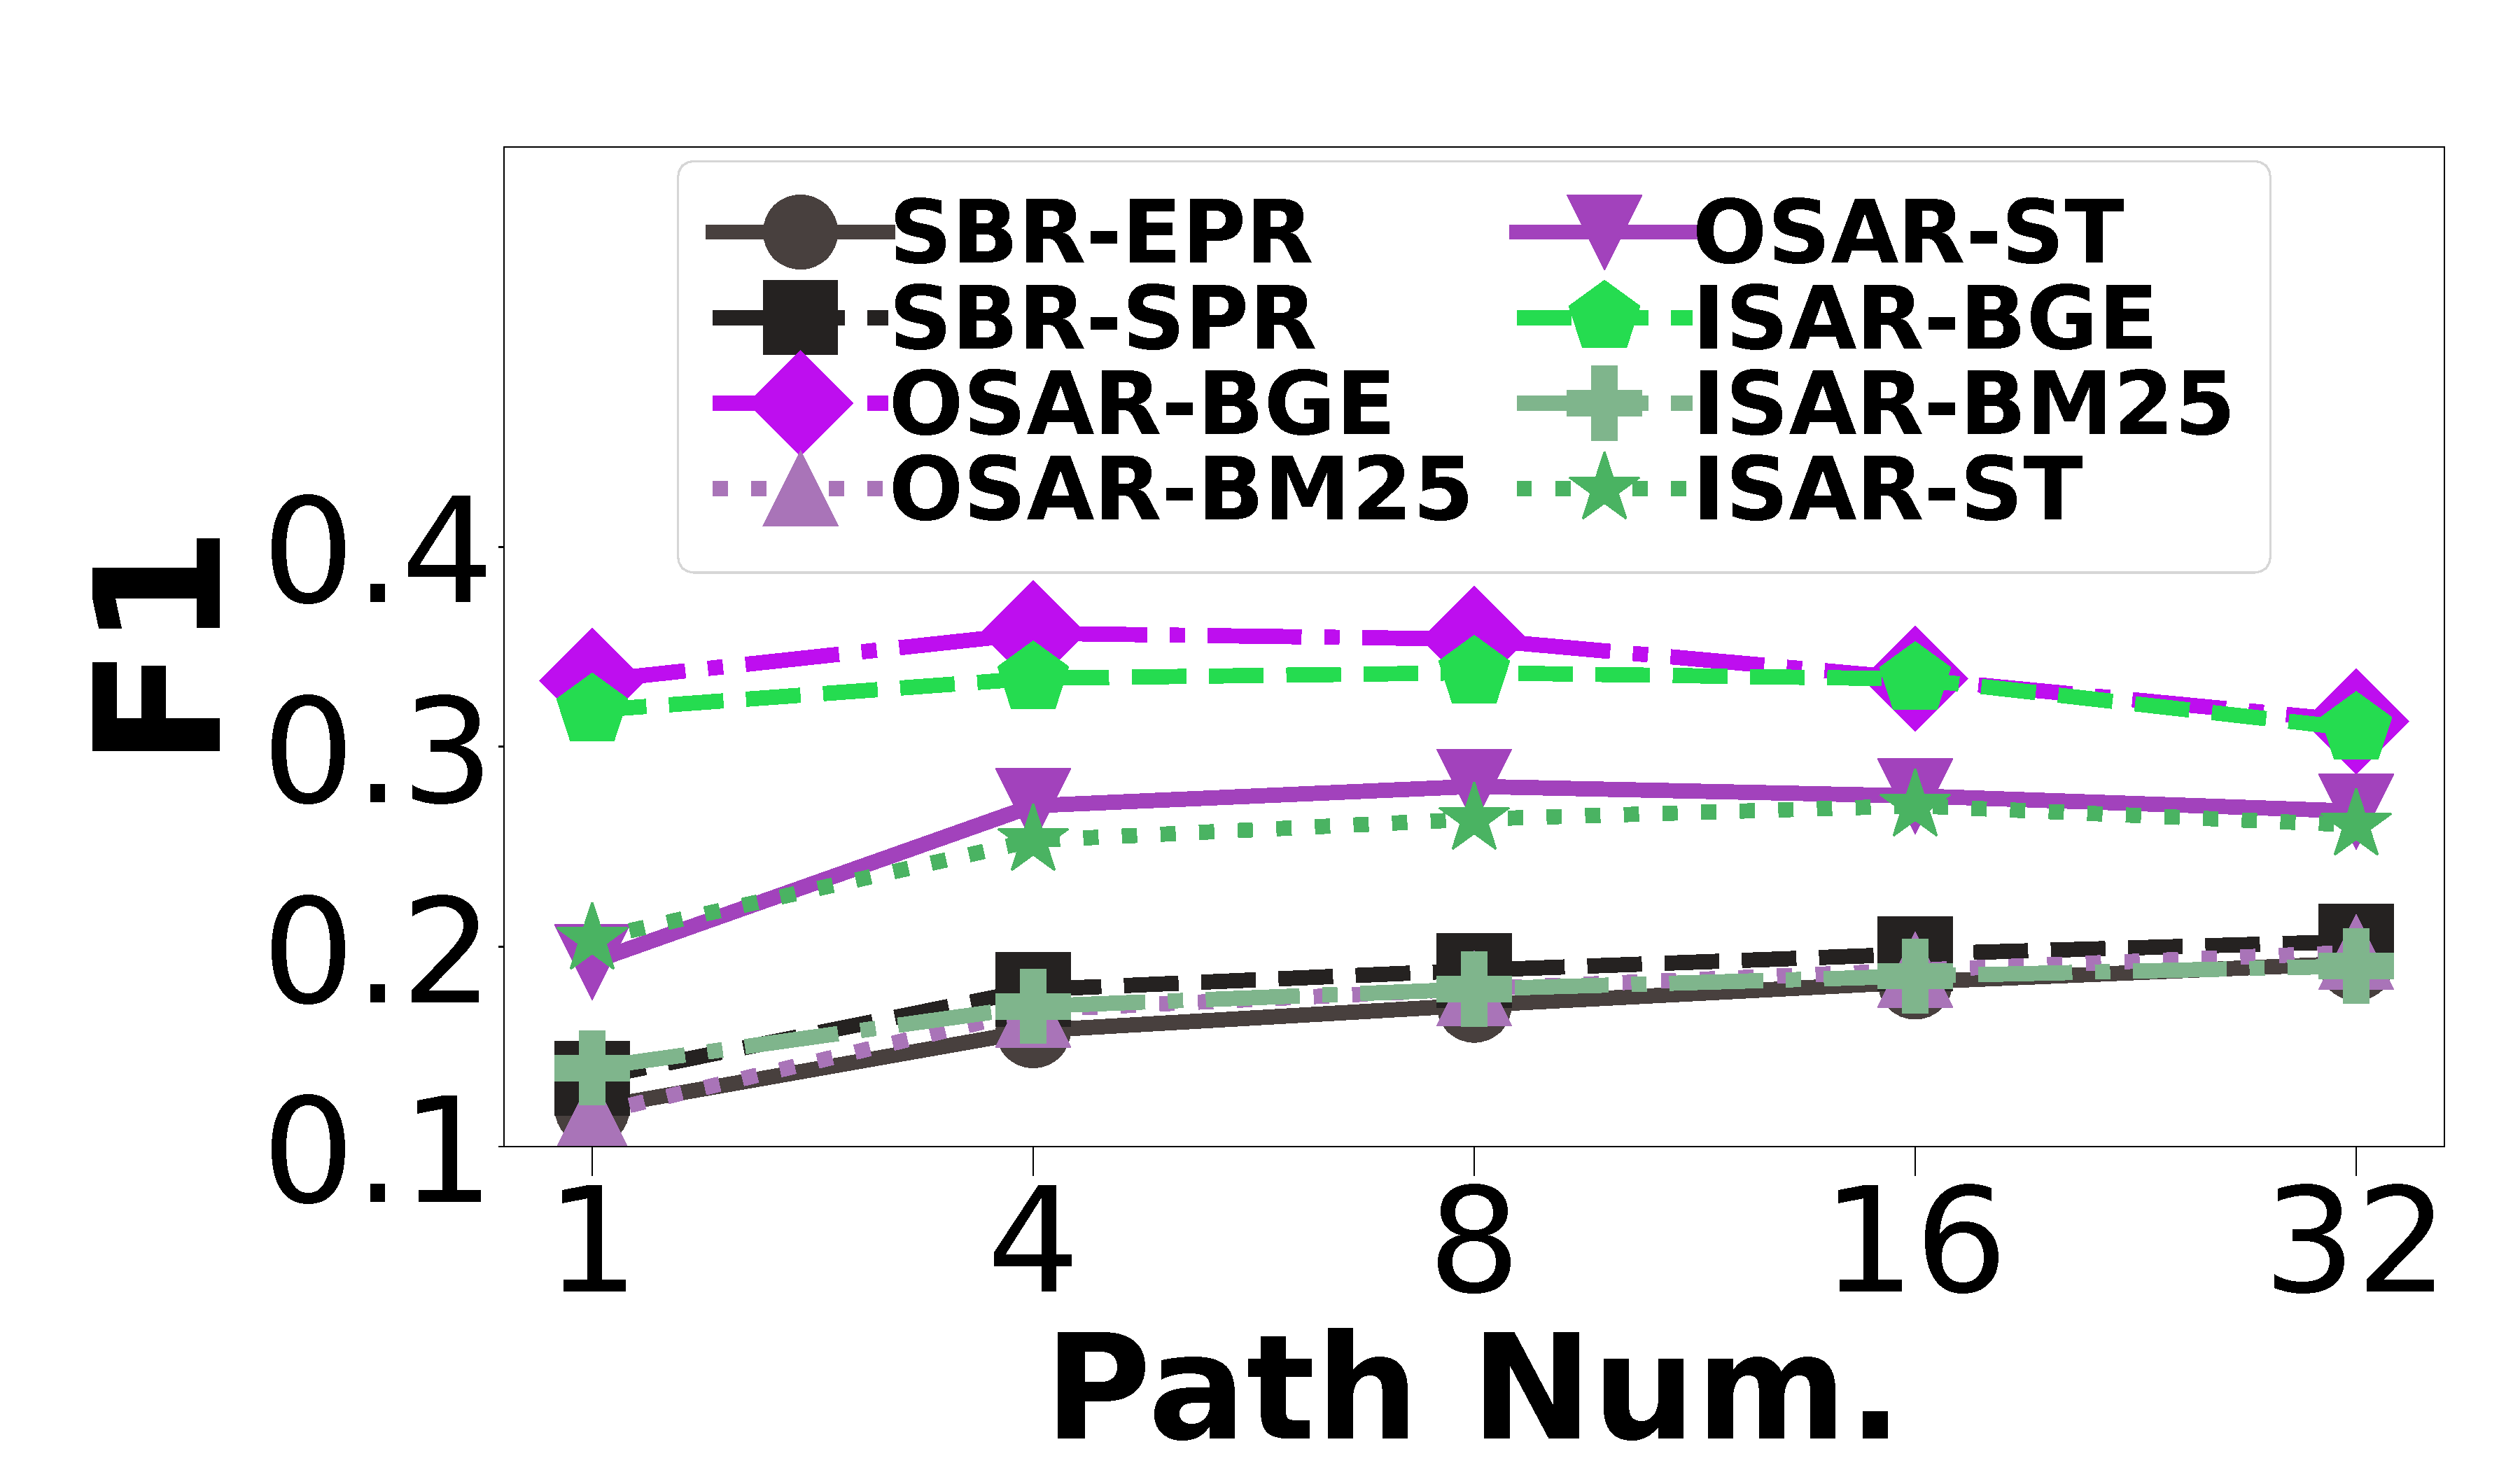
\includegraphics[width=\textwidth,height=2.3cm]{figures/PR/PR-Average-Merged.pdf}
        \vspace{-20pt}
        \caption{\small F1 Score vs. \# of Paths (for Methods of Path-Retrieval)}
        %\vspace{-10pt}
        \label{fig:PR-F1}

    \end{minipage}%
    \hspace{0.1cm}
    \begin{minipage}{0.22\textwidth}
            \centering
        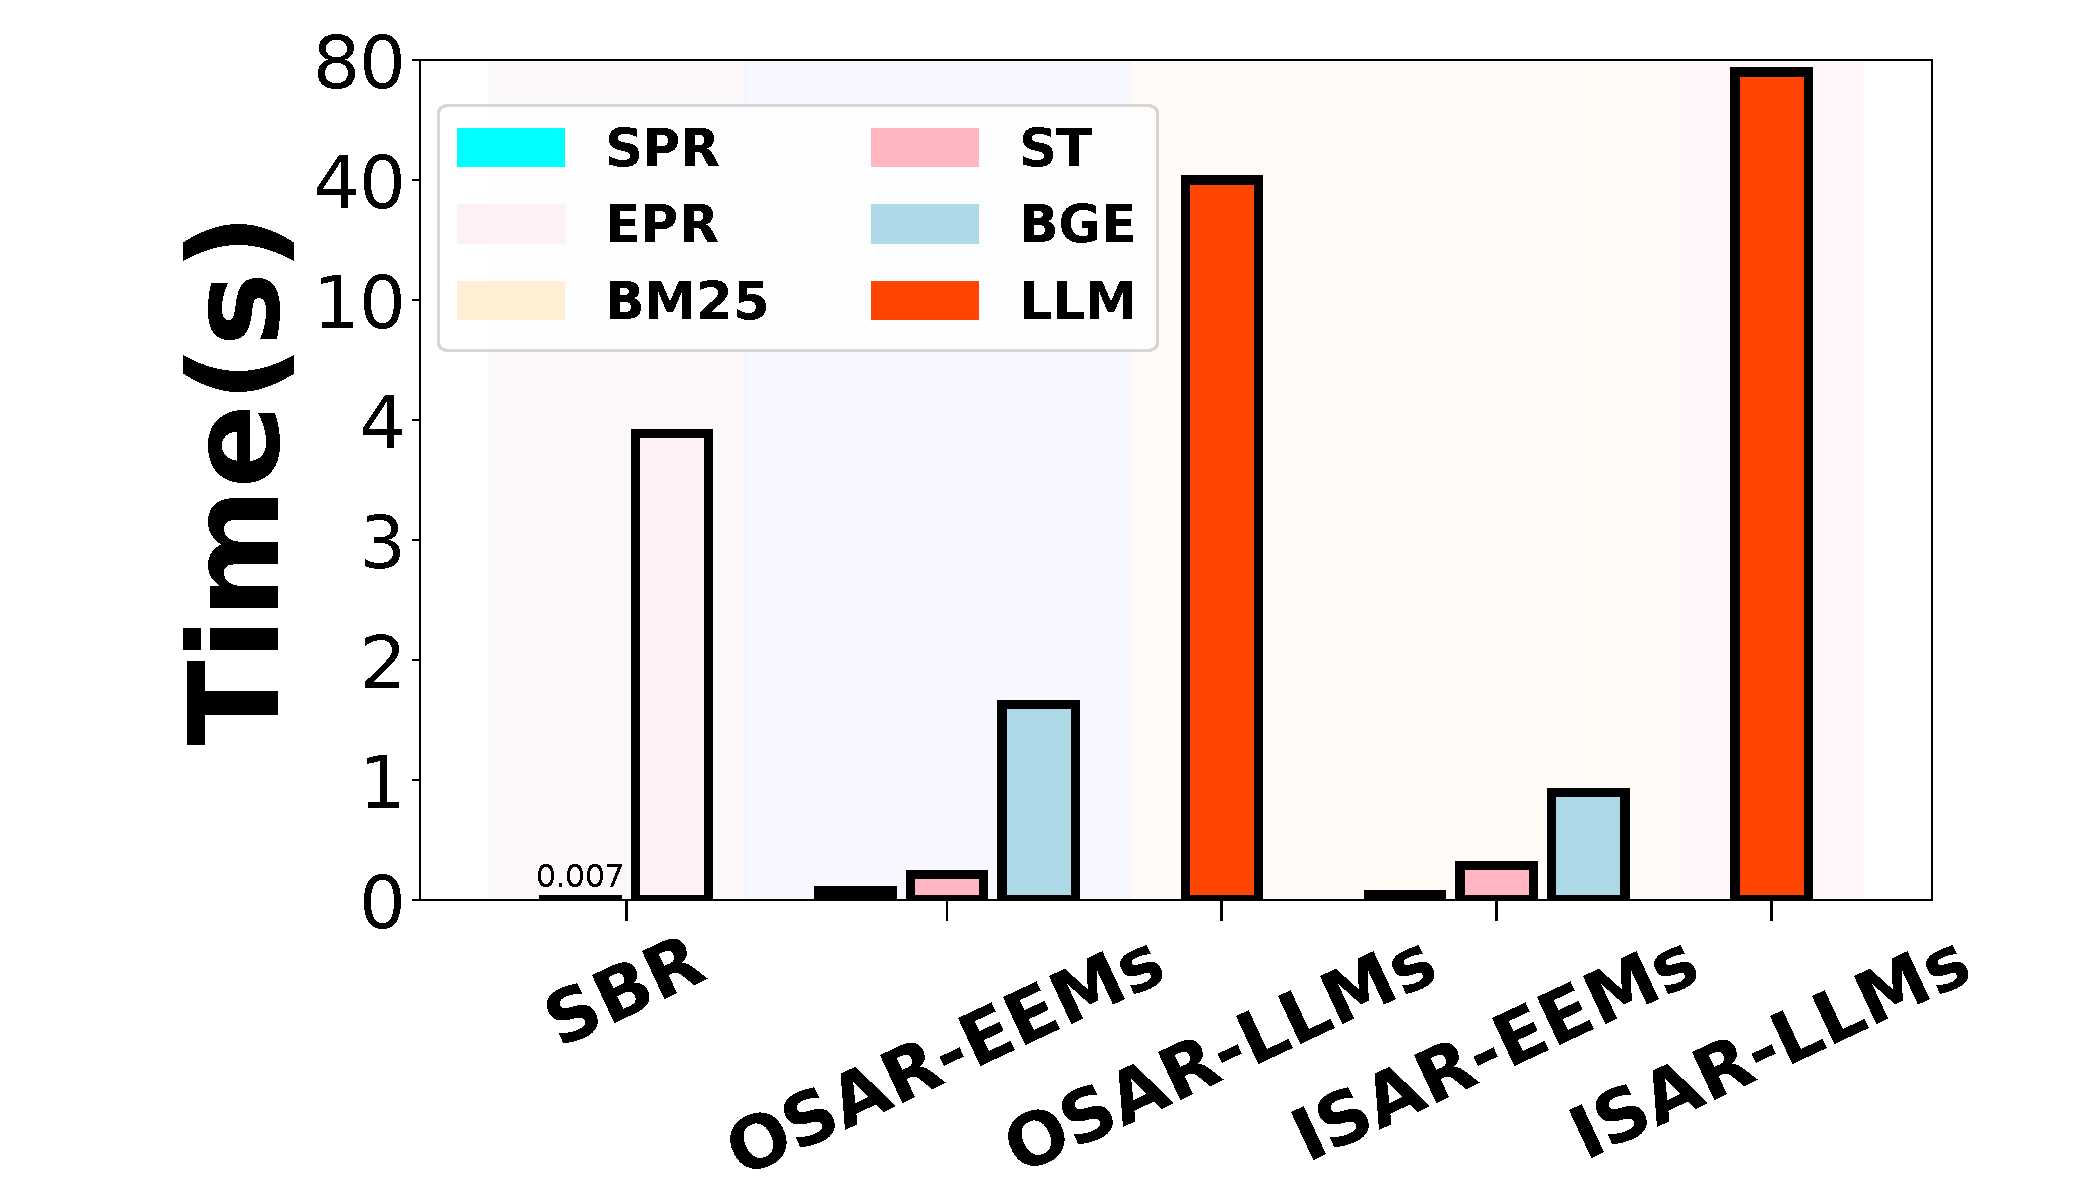
\includegraphics[width=\linewidth,height=2.1cm]{figures/PR/PR-Time.pdf}
        \vspace{-14pt}
        \caption{\small Runtime of Methods in Path-Retrieval {\small(WebQSP)}}
        \label{fig:PR-cost}
    \end{minipage}
    %\vspace{-10pt}
\end{figure}
%\vspace{-10pt}


Table~\ref{tab:ISAR_h} reports the results of hybrid ISAR methods combining EEMs and LLMs. All three methods outperform single-model baselines on most datasets, confirming the benefit of combining model strengths. Notably, the EEMs-S strategy yields the best results, suggesting that combining EEMs and LLMs helps reduce the risk of missing important paths during expansion.



% \end{comment}
%To balance quality and efficiency, we recommend using ST as the representative model for EEMs.%, ensuring a effective solution.
%the batch size of BGE and ST is set to 64 and the max input token of LLMs is set to 16k